\documentclass[9pt]{beamer}


\def\Title{Bayesian machine learning\\\vspace{3mm}
Bayesian deep learning}

\usepackage{natbib}
\usetheme[height=0mm]{Rochester}
\usecolortheme{}
\usefonttheme[onlylarge]{structurebold}
\setbeamerfont*{frametitle}{size=\normalsize,series=\bfseries}
\setbeamertemplate{navigation symbols}{}
\setbeamercovered{dynamic}
\setbeamertemplate{itemize item}[triangle]
\setbeamertemplate{itemize subitem}[triangle]

%  use Darmstadt if commenting the next line
\usepackage[footheight=1em]{beamerthemeboxes}
\usepackage[natbib=true,backend=biber,citestyle=authoryear,maxbibnames=2]{biblatex}
\bibliography{../bib/biblio_julyan} % ../bib/stats,../bib/statsjulyan,../bib/learningjulyan

%\let\oldcite=\cite
%\renewcommand\cite[1]{\hyperlink{#1}{\textcolor{gray}{\oldcite{#1}}}}
%\let\oldcite=\citet
%\renewcommand\citet[1]{\hyperlink{#1}{\textcolor{gray}{\oldcite{#1}}}}
%\let\oldcitep=\citep
%\renewcommand\citep[1]{\hyperlink{#1}{\textcolor{gray}{\oldcitep{#1}}}}

\usepackage{amsmath,amssymb,amsthm,bbm}             % AMS Math
\usepackage[utf8]{inputenc}
\usepackage[english]{babel}
%\usepackage{myAlgorithm}
\usepackage{xcolor}
\usepackage{graphicx}
\usepackage{subfigure}
\usepackage{hyperref}
\usepackage{mathtools}
\usepackage{mathrsfs}
\usepackage{animate}
%\usepackage{fontawesome5} % twitter bird


\usepackage{color}
%\usepackage[citecolor=blue]{hyperref}
%\RequirePackage[citecolor=blue]{hyperref}
%\usepackage{animate}
\usepackage{xspace}
\usepackage{algorithm, algorithmic}
\usepackage{mathrsfs,dsfont}
\usepackage{amssymb,amsmath,amsthm,graphicx}
\usepackage{animate}
%\graphicspath{{./Figures/}}
\usepackage{setspace} % with \setstretch{1.3}
\usepackage{yfonts}
%\usepackage[square]{natbib}
%\usepackage{graphicx}

% packages on graphs and tables
\usepackage{booktabs}
\setlength{\heavyrulewidth}{1.5pt}
\setlength{\abovetopsep}{4pt}
\usepackage{rotating} % for tables


\usepackage{marvosym} % for website symbols
\usepackage{transparent}

\usepackage{appendixnumberbeamer} 

\usepackage{amsmath,amsthm}

\usepackage[export]{adjustbox}



\newtheorem{proposition}{Proposition}
\newtheorem{remark}{Remark}


\definecolor{forestgreen}{rgb}{0.13, 0.55, 0.13}
\definecolor{darkblue}{rgb}{0.0, 0.0, 0.65}
\definecolor{violet2}{rgb}{0.5,0,0.5}
\definecolor{orange2}{rgb}{0.8, 0.1, 0.1}       
\definecolor{red2}{rgb}{1, 0.4, 0}

\hypersetup{
	colorlinks=true,
	urlcolor=orange2,
	citecolor=orange2,
	linktoc=all,
	linkcolor=orange2}

\allowdisplaybreaks
%\renewcommand{\alert}[1]{\textcolor{red2}{#1}}
\newcommand{\question}[1]{\textcolor{forestgreen}{#1}}



\setbeamertemplate{footline}[frame number]


%%%%%%%%%%%%%%%%%
% see option in Beamer guide, section 10: https://tug.ctan.org/macros/latex/contrib/beamer/doc/beameruserguide.pdf
\AtBeginSection[] % Do nothing for \section*
{
\begin{frame}
\frametitle{Outline}
\tableofcontents[currentsection,
				 hideothersubsections]
\end{frame}
}


\AtBeginSubsection[] % Do nothing for \section*
{
\begin{frame}
\frametitle{Outline}
\tableofcontents[currentsection,
				subsectionstyle=show/shaded/hide,
				subsubsectionstyle=hide
%				currentsubsection,
%				hideothersubsections,
%				hideothersubsubsections,
				%subsectionstyle=show/shaded
				]
\end{frame}
}

\newcommand{\backupbegin}{
   \newcounter{framenumberappendix}
   \setcounter{framenumberappendix}{\value{framenumber}}
}
\newcommand{\backupend}{
   \addtocounter{framenumberappendix}{-\value{framenumber}}
   \addtocounter{framenumber}{\value{framenumberappendix}}
}
\makeatletter

\title{\Title} 
\author[Julyan Arbel (Inria Grenoble Rh\^one-Alpes \& Univ. Grenoble-Alpes)] % (optional, for multiple authors)
{Julyan Arbel}
\institute[] % (optional)
{\normalsize 
 Statify team, Inria  Grenoble Rh\^one-Alpes \& Univ. Grenoble-Alpes, France\\
 \Letter \, \href{mailto:julyan.arbel@inria.fr}{julyan.arbel@inria.fr} \quad
%\Phone +39 329 32 38 810 
\ComputerMouse \, \href{http://www.julyanarbel.com}{www.julyanarbel.com} 
%\quad \faIcon{twitter} \, \href{https://twitter.com/JulyanArbel}{$@$JulyanArbel} 
\\
\vspace{.2cm}
\url{http://github.com/rbardenet/bml-course}\\
\vspace{1cm}\hspace{-4cm}

\includegraphics[width=0.3\textwidth]{figures_julyan/logo/inria.png}\\
\vspace{-2cm}\hspace{4.5cm}
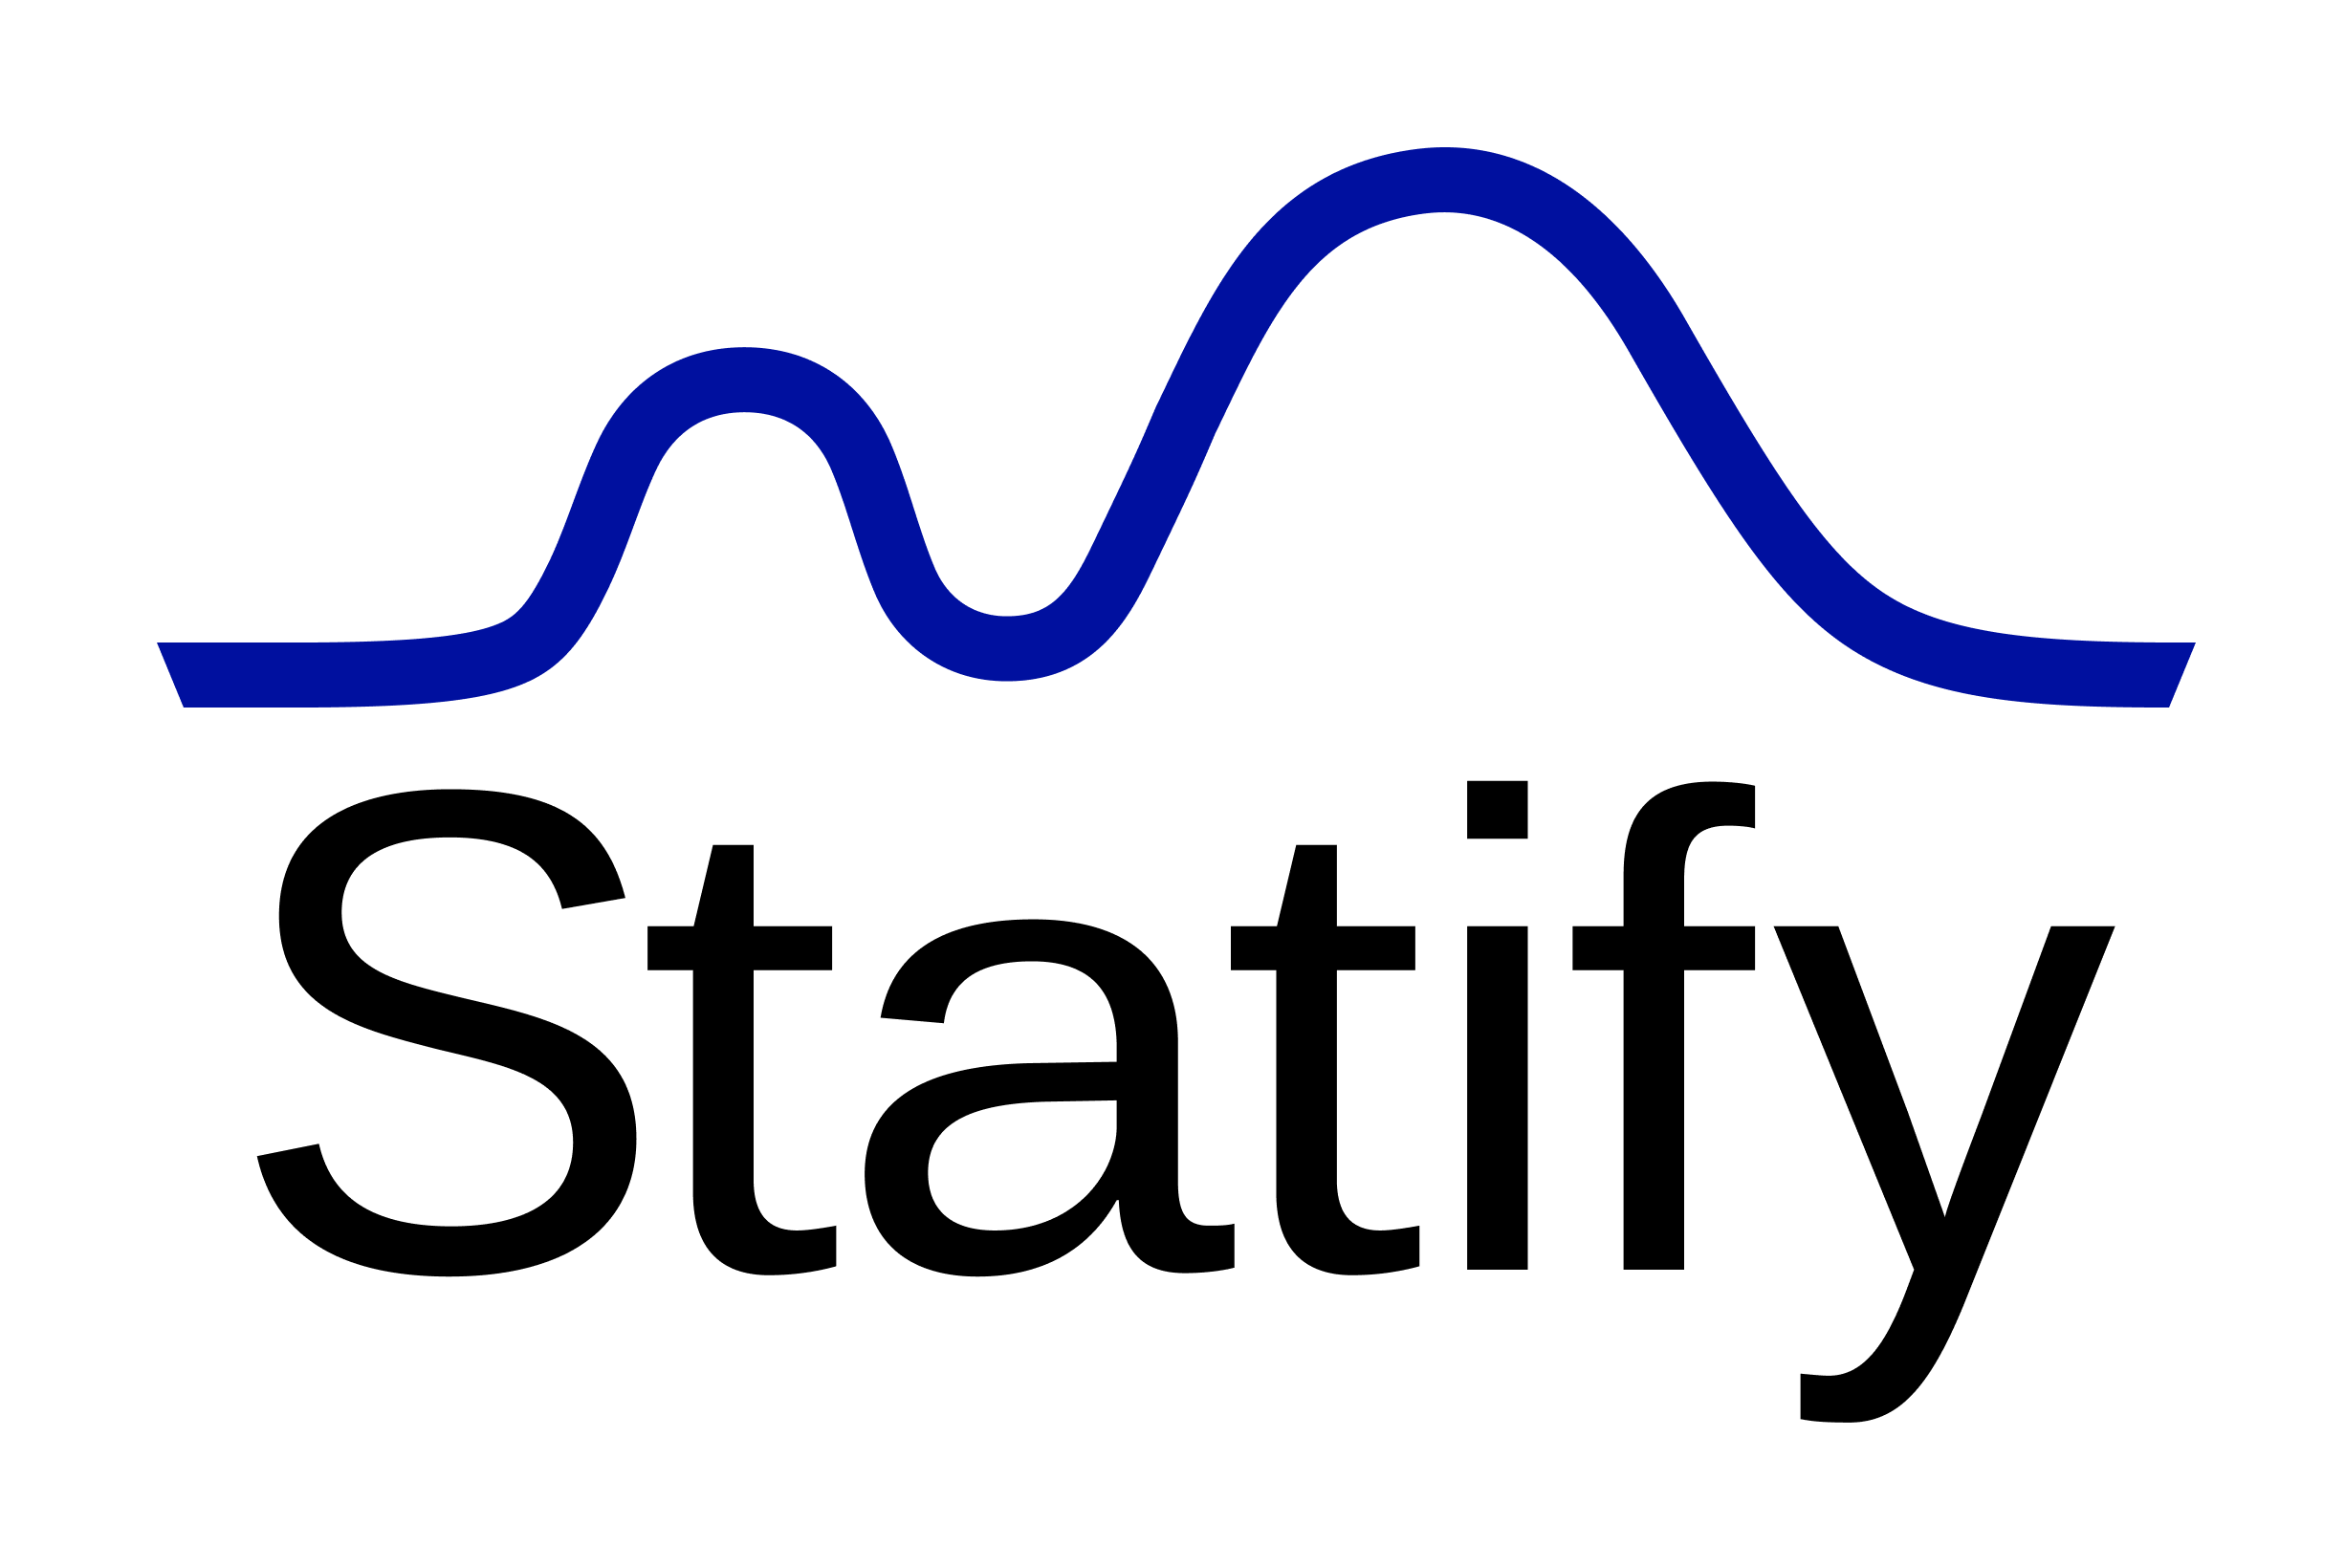
\includegraphics[width=0.3\textwidth]{figures_julyan/logo/statify.png}
}
\date{}



\definecolor{forestgreen}{rgb}{0.13, 0.55, 0.13}
\definecolor{darkblue}{rgb}{0.0, 0.0, 0.65}
\definecolor{violet2}{rgb}{0.5,0,0.5}
\definecolor{orange2}{rgb}{0.8, 0.1, 0.1}       
\definecolor{red2}{rgb}{1, 0.4, 0}






% specifics Julyan
\setlength{\parskip}{0.5\baselineskip}%
\setlength{\parindent}{0pt}%
% end specifics Julyan


\newcommand{\T}{{\text{\tiny\sffamily\upshape\mdseries T}}}
\newcommand{\bx}{\boldsymbol{x}}
\newcommand{\bmu}{\boldsymbol{\mu}}
\newcommand{\bh}{\boldsymbol{h}}
\newcommand{\bb}{\boldsymbol{b}}
\newcommand{\bV}{\boldsymbol{V}}
\newcommand{\bW}{\boldsymbol{W}}
%\newcommand{\bU}{\boldsymbol{U}}
\newcommand{\bH}{\boldsymbol{H}}
\newcommand{\bw}{\boldsymbol{w}}
\newcommand{\bz}{\boldsymbol{z}} 
\newcommand{\bX}{\boldsymbol{X}} 
\newcommand{\by}{\boldsymbol{y}} 
\newcommand{\bg}{\boldsymbol{g}} 
\newcommand{\bv}{\boldsymbol{v}} 
\newcommand{\be}{\boldsymbol{e}} 
\newcommand{\boldf}{\boldsymbol{f}} 
\newcommand{\Lnorm}{\mathcal{L}} 
\newcommand{\R}{\mathbb{L}} 
\newcommand{\subW}{subW} % \normalfont 

\def\simiid{\overset{\text{iid}}{\sim}}
\def\simind{\overset{\text{ind}}{\sim}}
%\newcommand{\ind}{\perp\!\!\!\!\perp} 

% for BNP part

%% Michal's

\newcommand{\PrecisionParam}{\alpha}
\newcommand{\Dir}{\text{Dir}}
\newcommand{\Beta}{\text{Beta}}

\usepackage{mathtools}

\newcommand\diseq{\stackrel{\mathclap{\normalfont\mbox{\small{d}}}}{=}}


%\newcommand{\distas}[1]{\mathbin{\overset{#1}{\kern\z@\sim}}}%
\newsavebox{\mybox}\newsavebox{\mysim}
\newcommand{\distras}[1]{%
  \savebox{\mybox}{\hbox{\kern3pt$\scriptstyle#1$\kern3pt}}%
  \savebox{\mysim}{\hbox{$\sim$}}%
  \mathbin{\overset{#1}{\kern\z@\resizebox{\wd\mybox}{\ht\mysim}{$\sim$}}}%
}


%% mathbb
\newcommand{\bbC}{\mathbb{C}}
\newcommand{\indic}{\mathds{1}}
\newcommand{\F}{\mathbb{F}}
\newcommand{\X}{\mathbb{X}}
%\newcommand{\Z}{\mathbb{Z}}
\newcommand{\Sd}{\mathbb{S}}
\newcommand{\Y}{\mathbb{Y}}


%% mathds
%\newcommand{\R}{\mathbb{R}}
\newcommand{\E}{\mathrm{E}}
\newcommand{\Cov}{\mathsf{Cov}}
\newcommand{\Var}{\mathsf{Var}}
\newcommand{\N}{\mathds{N}}
\newcommand{\Nbb}{\mathds{N}}
\renewcommand{\P}{\mathds{P}}

\newcommand{\Xn}{X^n}



%%% Script letters
\newcommand{\Bcr}{\mathscr{B}}
\newcommand{\Fcr}{\mathscr{F}}
\newcommand{\Dcr}{\mathscr{D}}
\newcommand{\Icr}{\mathscr{I}}
\newcommand{\Lcr}{\mathscr{L}}
\newcommand{\Pcr}{\mathscr{P}}
\newcommand{\Xcr}{\mathscr{X}}
\newcommand{\Mcr}{\mathscr{M}}
\newcommand{\Ycr}{\mathscr{Y}}
\newcommand{\Acr}{\mathscr{A}}
\newcommand{\Gcr}{\mathscr{G}}
\newcommand{\Vcr}{\mathscr{V}}

%%% Mathfrak
\newcommand{\Xf}{\mathfrak{X}}
\newcommand{\Sf}{\mathfrak{\sigma}}

\newcommand{\ddr}{\mathrm{d}}
\newcommand{\edr}{\mathrm{e}}
\newcommand{\idr}{\mathrm{i}}

%\renewcommand{\abstractname}{SUMMARY}
\renewcommand{\theparagraph}{\arabic{paragraph}}
%\numberwithin{equation}{paragraph}

\newcommand{\Rt}{\Rightarrow}
\newcommand{\rt}{\rightarrow}
\newcommand{\lrt}{\longrightarrow}
\newcommand{\Lerit}{\Leftrightarrow}
\newcommand{\dimo}{\underline{\textsc{Proof.}} }
\newcommand{\cc}{\hfill $\square$}
\newcommand{\ind}{\bm 1}
\newcommand{\bm}{\mathbf}
\newcommand{\var}{\varepsilon}
\newcommand{\intre}{\int_{\mathbb{R}}}
\newcommand{\intoinf}{\int_0^{+\infty}}

\newcommand{\Bc}{\mathcal{B}}
\newcommand{\Cc}{\mathcal{C}}
\newcommand{\Fc}{\mathcal{F}}
\newcommand{\Lc}{\mathcal{L}}
\newcommand{\Nc}{\mathcal{N}}
\newcommand{\Pc}{\mathcal{P}}
\newcommand{\Ic}{\mathcal{I}}
\newcommand{\Zc}{\mathcal{Z}}

\newcommand{\dir}{P_{\alpha}}
\newcommand{\ep}{\varepsilon}
\newcommand{\e}{\mathsf{E}}
\newcommand{\trunc}{{\sigma,\tau}}
%\newcommand{\p}{\mathbb{P}}
\newcommand{\prob}{\mathsf{P}}
\newcommand{\Ga}{\Gamma_\alpha}
\newcommand{\Ma}{M_\alpha}
\newcommand{\Ua}{U_\alpha}
\newcommand{\Va}{V_\alpha}
\newcommand{\wt}{\widetilde}

\def\simind{\stackrel{\mbox{\scriptsize{ind}}}{\sim}}
\def\simiid{\stackrel{\mbox{\scriptsize{iid}}}{\sim}}

% altro
\newcommand{\mt}{{\mu}} % misura completamente aleatoria (CRM)
\newcommand{\hti}{{h}}
\newcommand{\St}{{S}}
\newcommand{\pt}{\tilde{p}} % legge aleatoria
\newcommand{\At}{\tilde{A}} %
\newcommand{\Bt}{\tilde{B}} %
\newcommand{\Lz}{\mathcal{L}_Z} % legge di Z

\newcommand{\AC}{\\[7pt]} % a capo
\newcommand{\La}{\mathcal{L}}
%\newcommand{\p}{\mathbb{P}}
%\newcommand{\AC}{\\[7pt]}
\newcommand{\bn}{\bar{n}}
\newcommand{\I}{\mathcal{I}}
\newcommand{\C}{\mathcal{C}}
\newcommand{\Ac}{\mathcal{A}}

% Ju
\newcommand{\vertju}{\,\vert\,}
\newcommand{\twoPD}{two-parameter Poisson-Dirichlet process\xspace}
\newcommand{\DP}{\text{Dirichlet process}\xspace}
\newcommand{\levy}{L\'evy\xspace}
\newcommand{\Gumbel}{\text{Gumbel}\xspace}
\newcommand{\Exp}{\text{Exp}\xspace}
\def\simiid{\stackrel{\mbox{\scriptsize{iid}}}{\sim}}
\def\simind{\stackrel{\mbox{\scriptsize{ind}}}{\sim}}
\def\proptoind{\stackrel{\mbox{\scriptsize{ind}}}{\propto}}
\newcommand{\citp}[1]{\textcolor{blue}{\citep{#1}}}
\newcommand{\citt}[1]{\textcolor{blue}{\citet{#1}}}


\newcommand{\crms}{completely random measures\xspace}
\newcommand{\crm}{completely random measure\xspace}
\newcommand{\CRM}{CRM\xspace}
\newcommand{\Crms}{Completely random measures\xspace}
\newcommand{\Crm}{Completely random measure\xspace}
\newcommand{\muA}{\tilde \mu(A)\xspace}
\newcommand{\muX}{\tilde \mu(\X)\xspace}
\newcommand{\cnkpar}{\binom{n}{k_1\cdots k_n}}
\newcommand{\cnkfact}{\frac{n!}{k_1!\ldots k_n!}}
\newcommand{\g}{\mathbf{g}}
\newcommand{\FK}{\citeauthor{ferguson1972representation}\xspace} 
\newcommand{\FKa}{\citeauthor{ferguson1972representation} algorithm\xspace} 
\newcommand{\BP}{\ensuremath{\text{BP}}\xspace} 
\newcommand{\BeP}{\ensuremath{\text{BeP}}\xspace} 
%\newcommand{\gg}{\ensuremath{\text{GG}}\xspace} 
\newcommand{\GG}{generalized gamma process\xspace} 
\newcommand{\SBP}{stable-beta process\xspace} 
\newcommand{\IBP}{Indian buffet process\xspace} 
\newcommand{\IG}{inverse-Gaussian process\xspace} 
\newcommand{\NMC}{N_{\text{\tiny{FK}}}} 
\newcommand{\EFK}{\mathbb{E}_{\text{\tiny{FK}}}}


\def\unit{\mathbf{1}}
\def\bc{c}
\def\prob{\mathbb{P}}
\def\bc{c}
\def\Ac{\mathcal{A}}
\def\VI{\text{VI}}
\def\En{\text{H}}
\def\B{\text{B}}
%\def\argmax{\text{argmax}}
\DeclareMathOperator*{\argmax}{arg\,max}
\DeclareMathOperator*{\argmin}{arg\,min}
\def\1{\unit}


%% notation
\DeclareMathOperator*{\argmax}{arg\,max}
\DeclareMathOperator*{\argmin}{arg\,min}
\newcommand{\cA}{\mathcal{A}}
\newcommand{\cS}{\mathcal{S}}
\newcommand{\cF}{\mathcal{F}}
\newcommand{\cX}{\mathcal{X}}
\newcommand{\cY}{\mathcal{Y}}
\newcommand{\cZ}{\mathcal{Z}}
\newcommand{\cN}{\mathcal{N}}
\newcommand{\cO}{\mathcal{O}}
\renewcommand{\leq}{\leqslant}
\renewcommand{\geq}{\geqslant}
\renewcommand{\phi}{\varphi}
\renewcommand{\epsilon}{\varepsilon}
\renewcommand{\d}{ {\rm d}}
\renewcommand{\emptyset}{\varnothing}


\usepackage{tikz}
\usepackage{tikzscale}
\usepackage{tcolorbox}

\usetikzlibrary{external}
%\tikzexternalize[mode=list and make, prefix=./, figure name=output-figure]

\usetikzlibrary{cd}
\tikzcdset{
  arrow style=tikz,
  diagrams={>={Straight Barb}}
}

\usetikzlibrary{patterns,positioning,arrows,shapes,shapes.geometric}
\usetikzlibrary{decorations,decorations.pathmorphing,intersections,backgrounds}

\usepackage{pgfplots}
\DeclareUnicodeCharacter{2212}{−}
\usepgfplotslibrary{groupplots,dateplot}
\usetikzlibrary{shapes.arrows}
\pgfplotsset{compat=newest}
\usepgfplotslibrary{groupplots}


\begin{document}
\begin{frame}
\maketitle
\end{frame}


\begin{frame}{Outline}
	\tableofcontents[pausesections,subsectionstyle=hide,subsubsectionstyle=hide]
\end{frame}


%%%%%%%%%%%%%%%%%%%%%%
\section{Introduction}
%%%%%%%%%%%%%%%%%%%%%%

%\begin{frame}{What comes to \emph{your} mind when you hear ``Bayesian deep learning''?}
%\end{frame}

%\begin{frame}{Deep neural networks}
%\begin{center}
%	\includegraphics[width=\textwidth]{figures_julyan/bnn}
%\end{center}
%\end{frame}


\begin{frame}{Deep neural networks Achilles heels}
\begin{center}
\only<1>{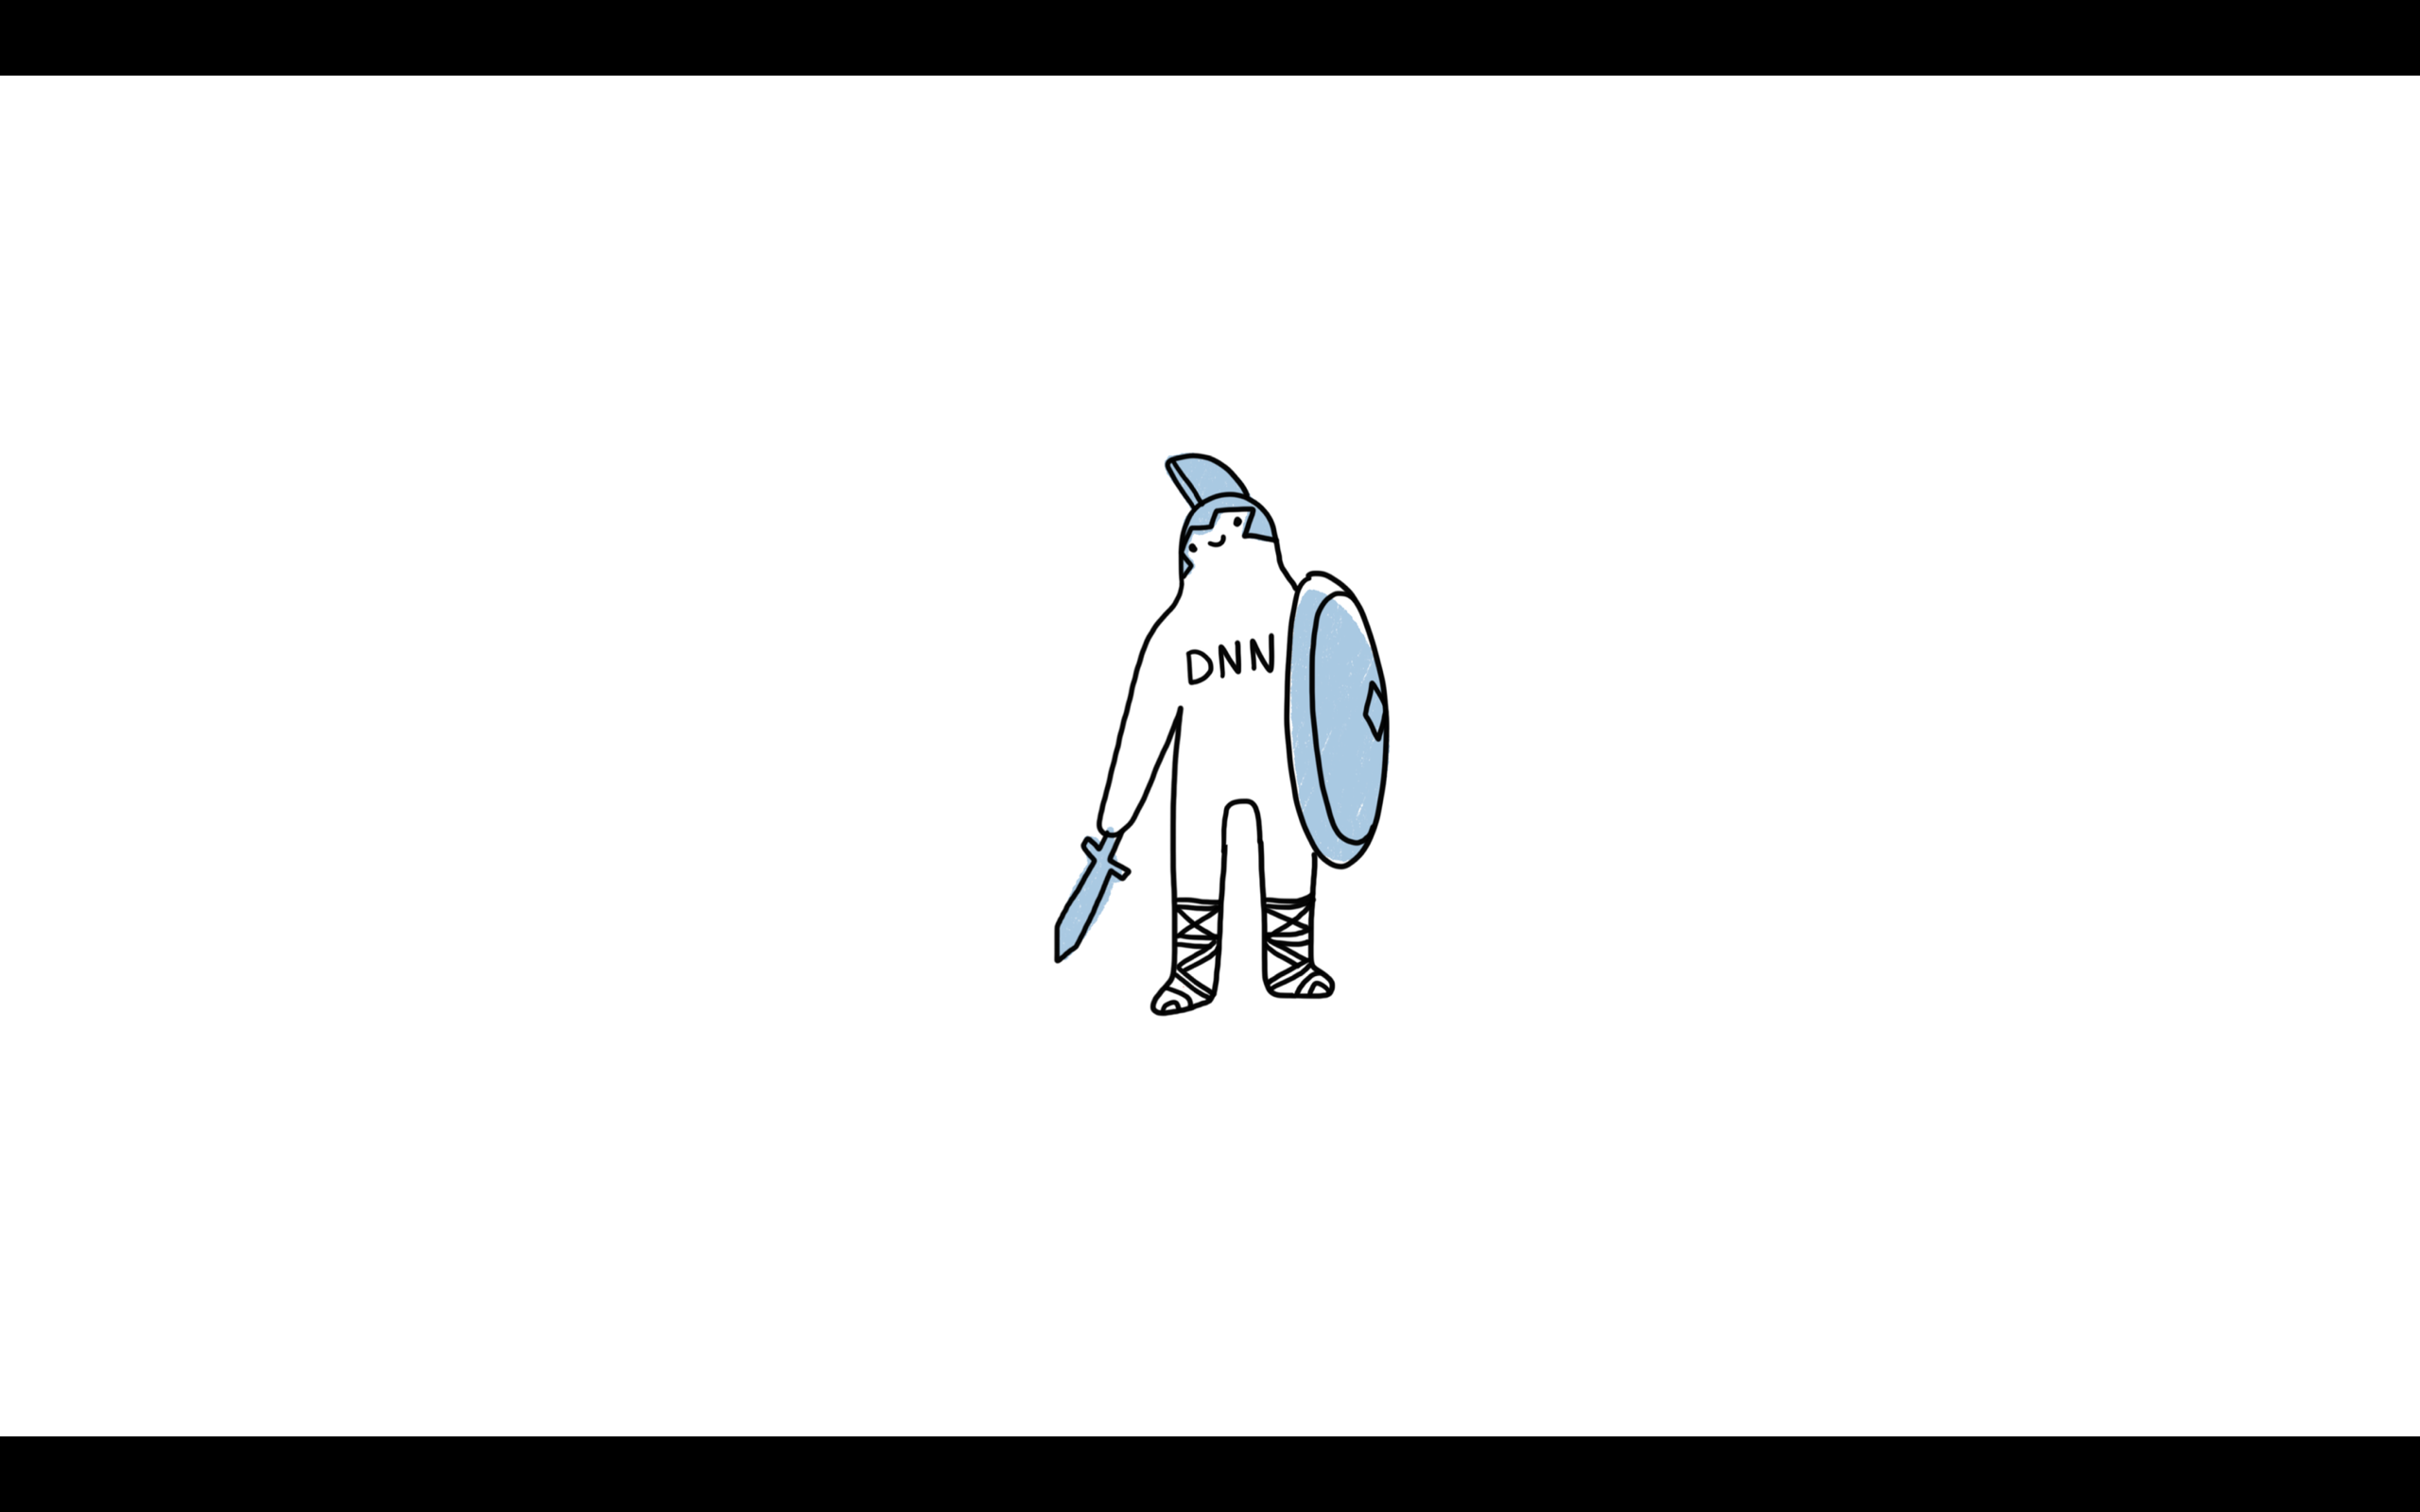
\includegraphics[height=.8\textheight,trim={12cm 6cm 12cm 8cm},clip]{figures_julyan/bdl/achilles1}}
\only<2>{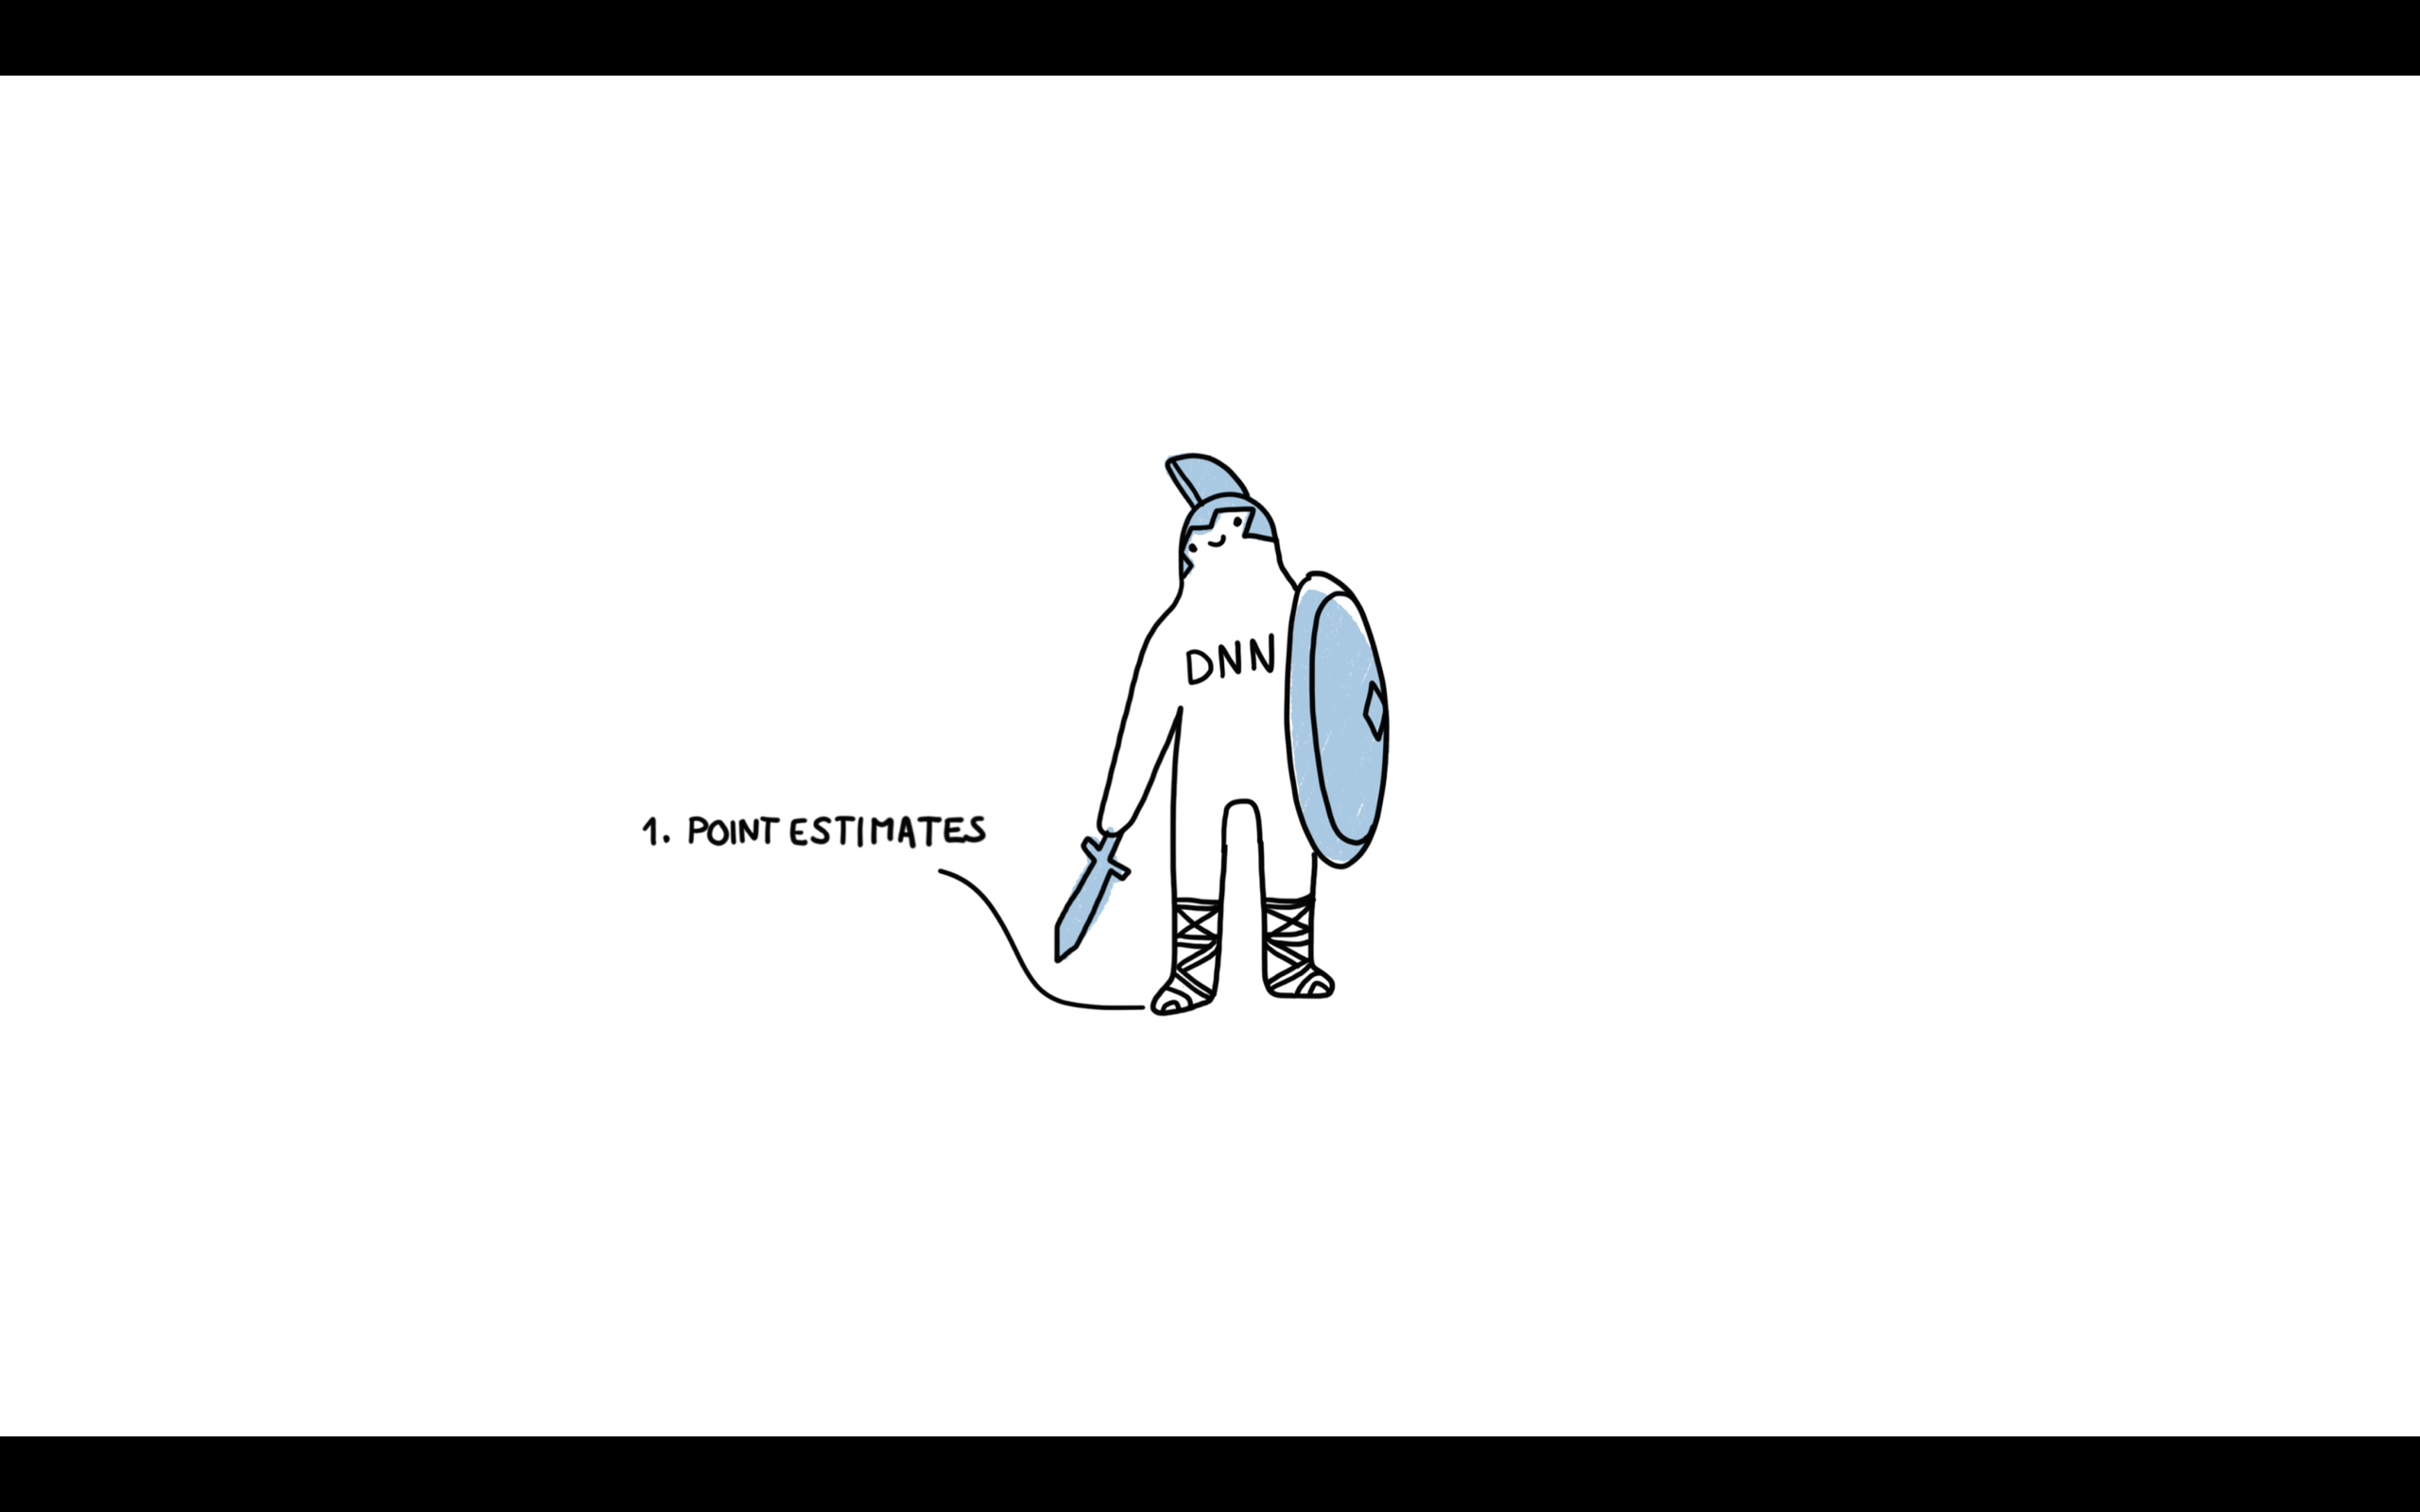
\includegraphics[height=.8\textheight,trim={12cm 6cm 12cm 8cm},clip]{figures_julyan/bdl/achilles2}}
\only<3>{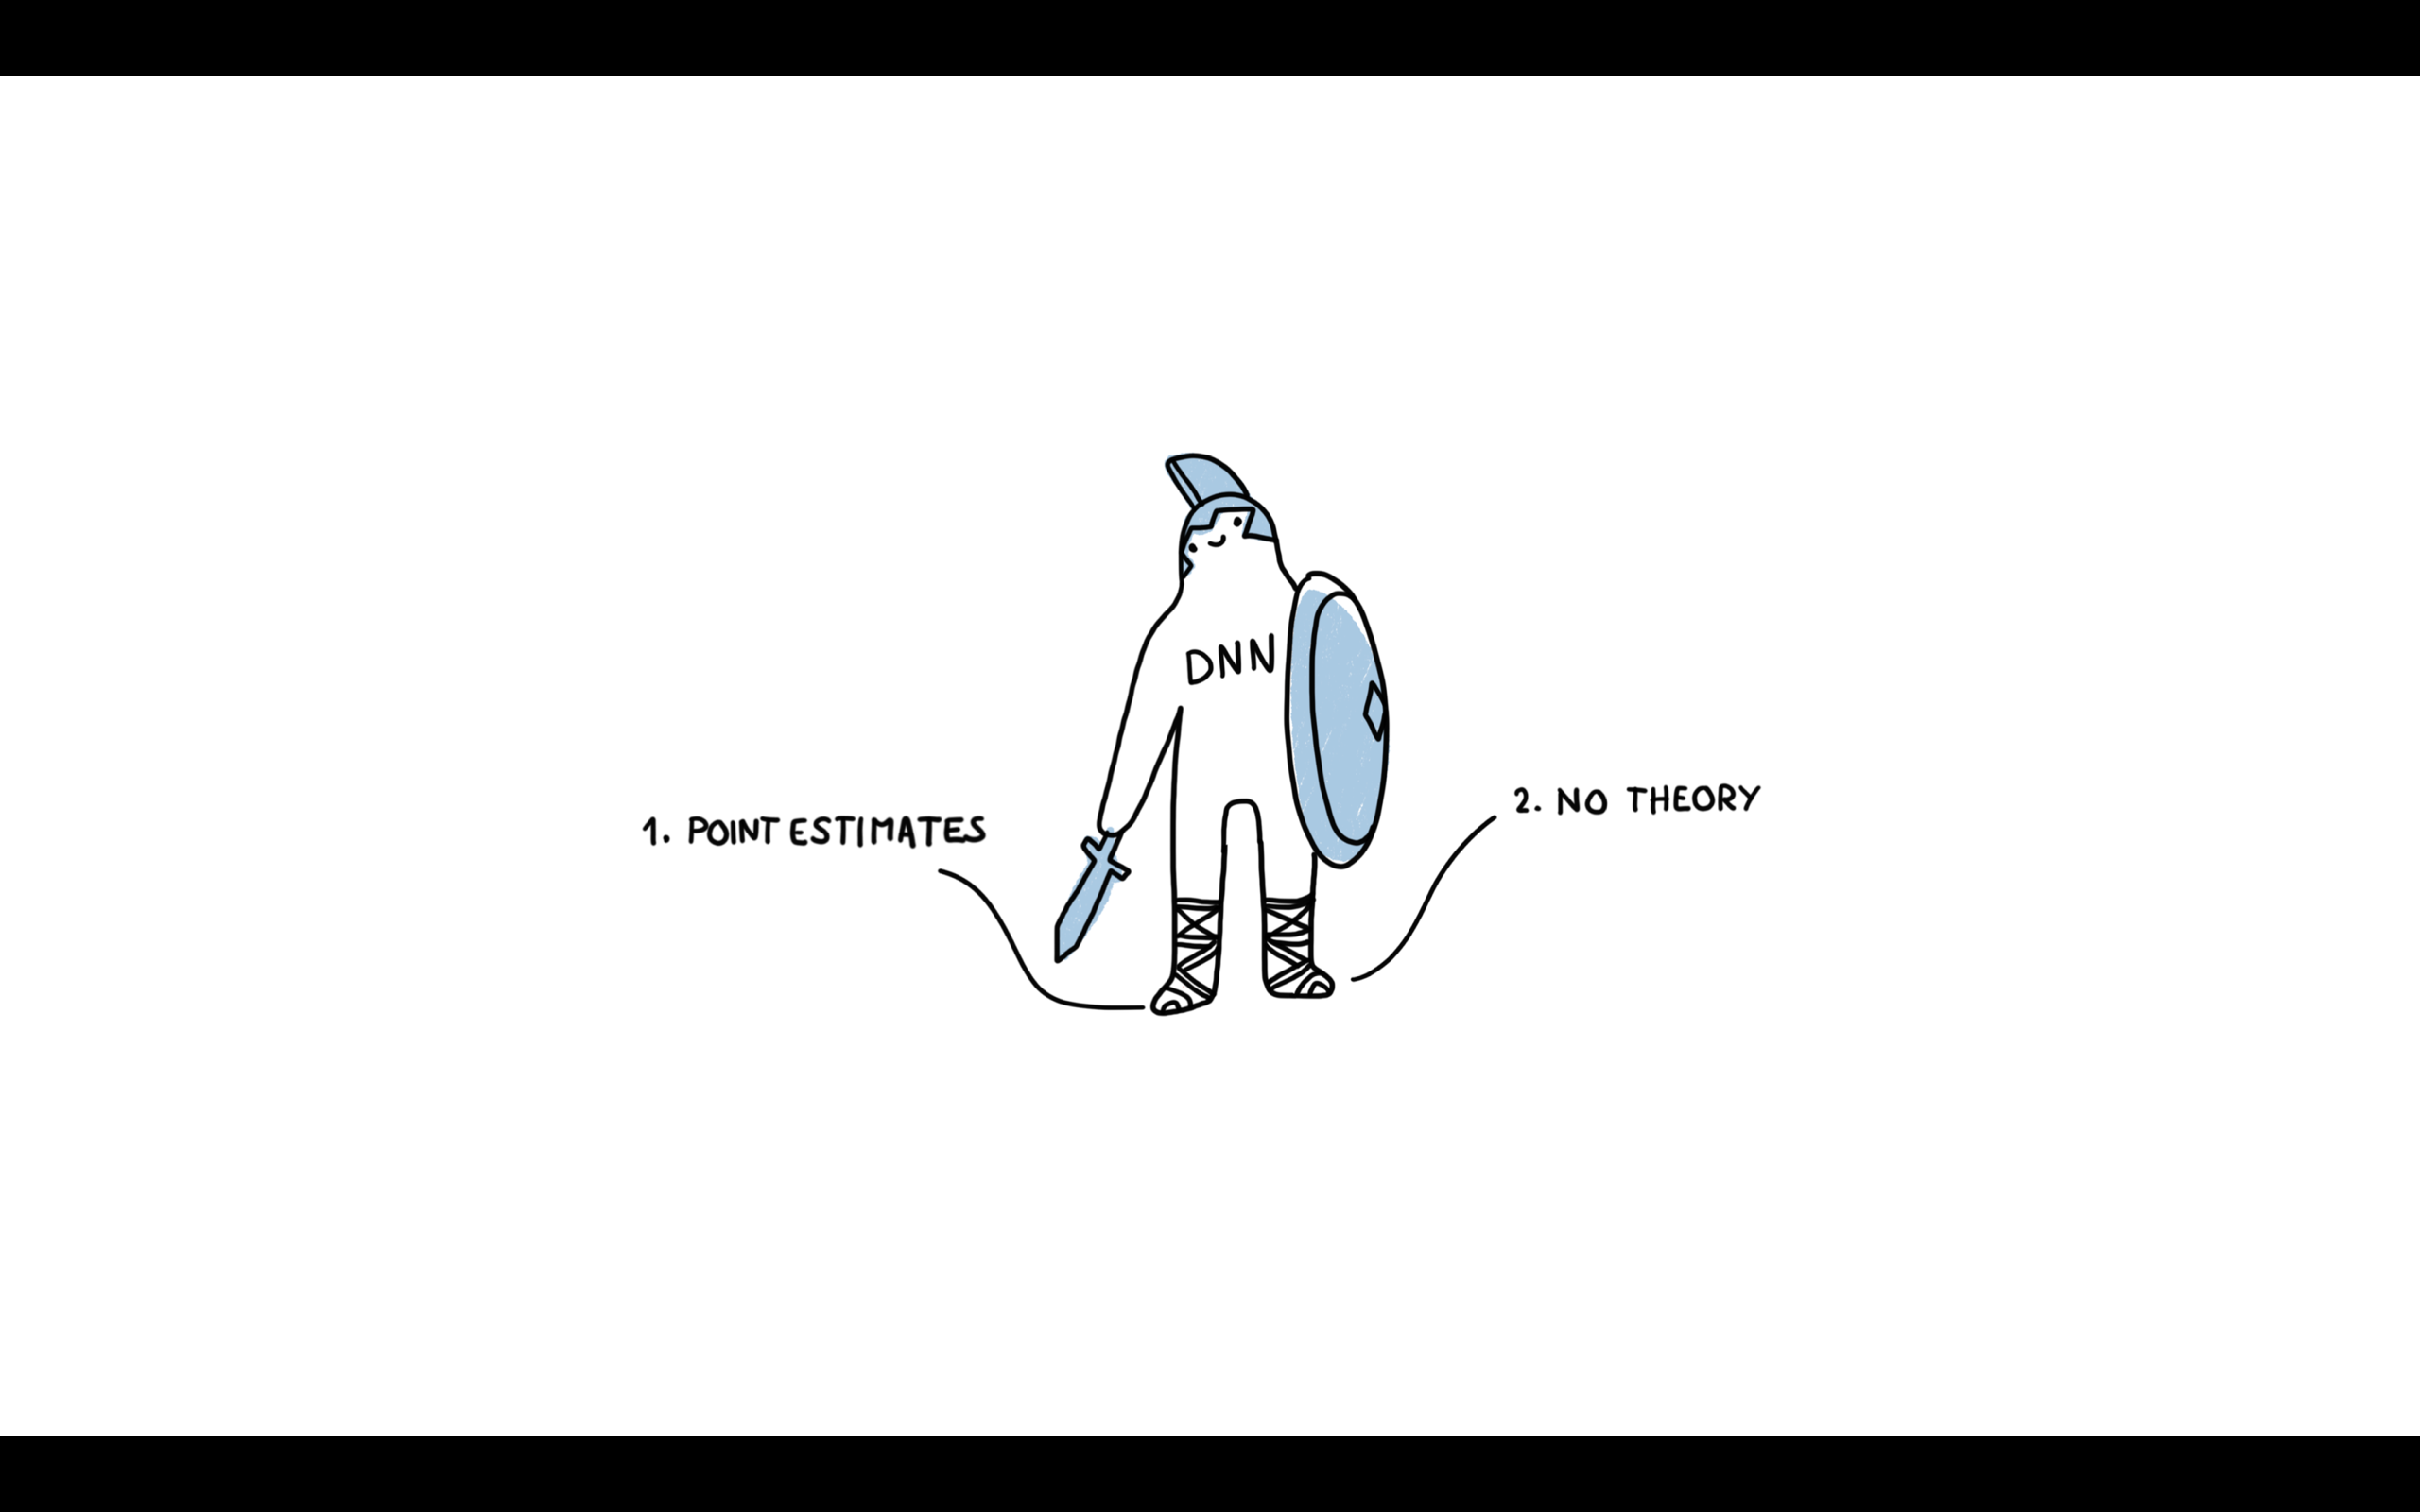
\includegraphics[height=.8\textheight,trim={12cm 6cm 12cm 8cm},clip]{figures_julyan/bdl/achilles3}}
\end{center}
\end{frame}

\begin{frame}{Different flavours of neural networks \citep{jospin2020handson}}
\begin{center}
\begin{tabular}{cc}
	\visible<1->{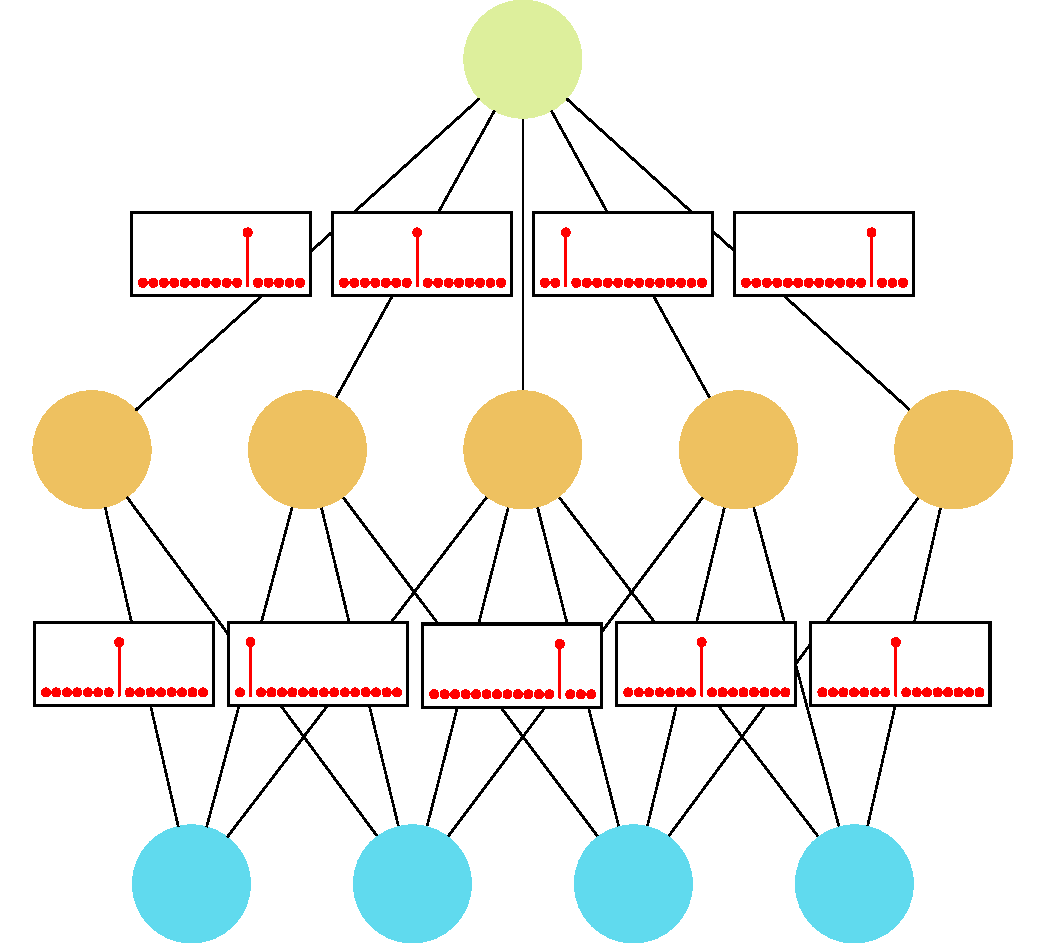
\includegraphics[width=.3\textwidth]{figures_julyan/bdl/hands-on/schemaNNPE}} &
	\visible<2->{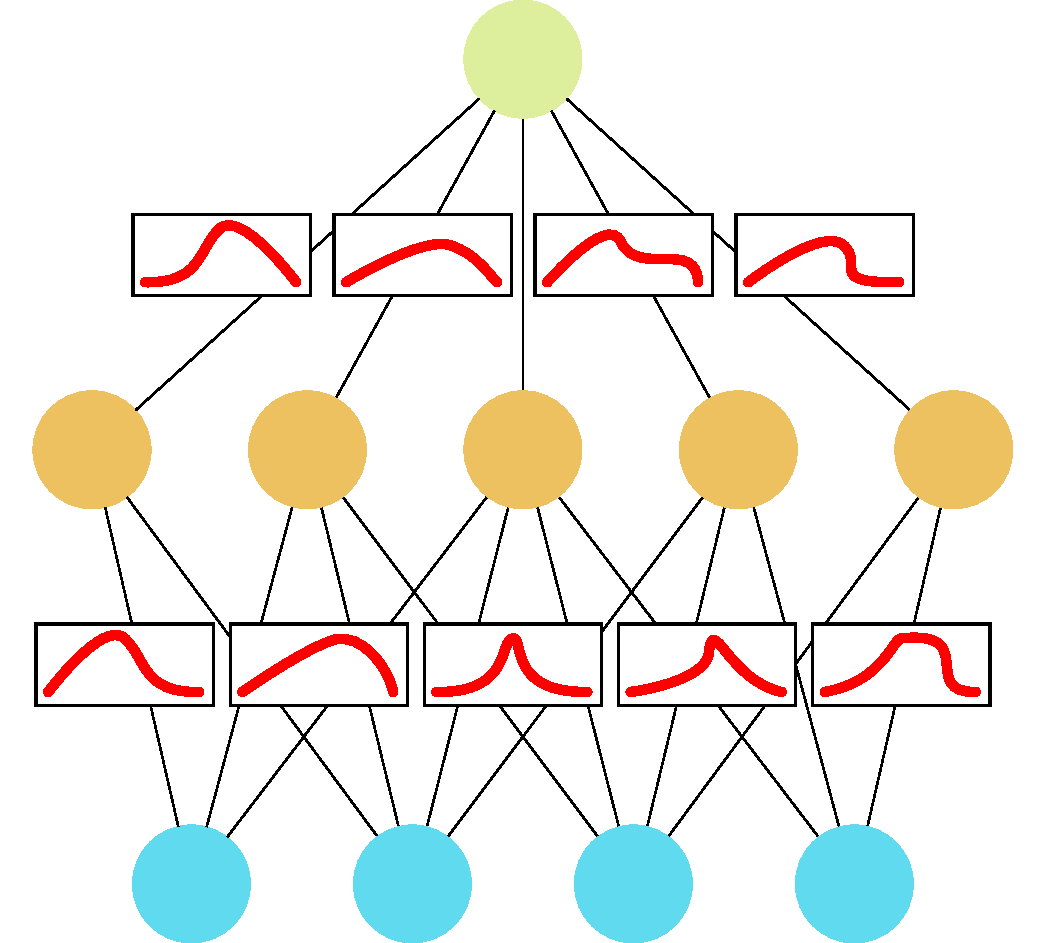
\includegraphics[width=.3\textwidth]{figures_julyan/bdl/hands-on/schemaNNStochastic}}\\
	\visible<1->{Neural networks} & 
	\visible<2->{Bayesian neural networks}\\
	\visible<1->{with point estimates} & 
	\visible<2->{with random weights}\\
	\visible<3->{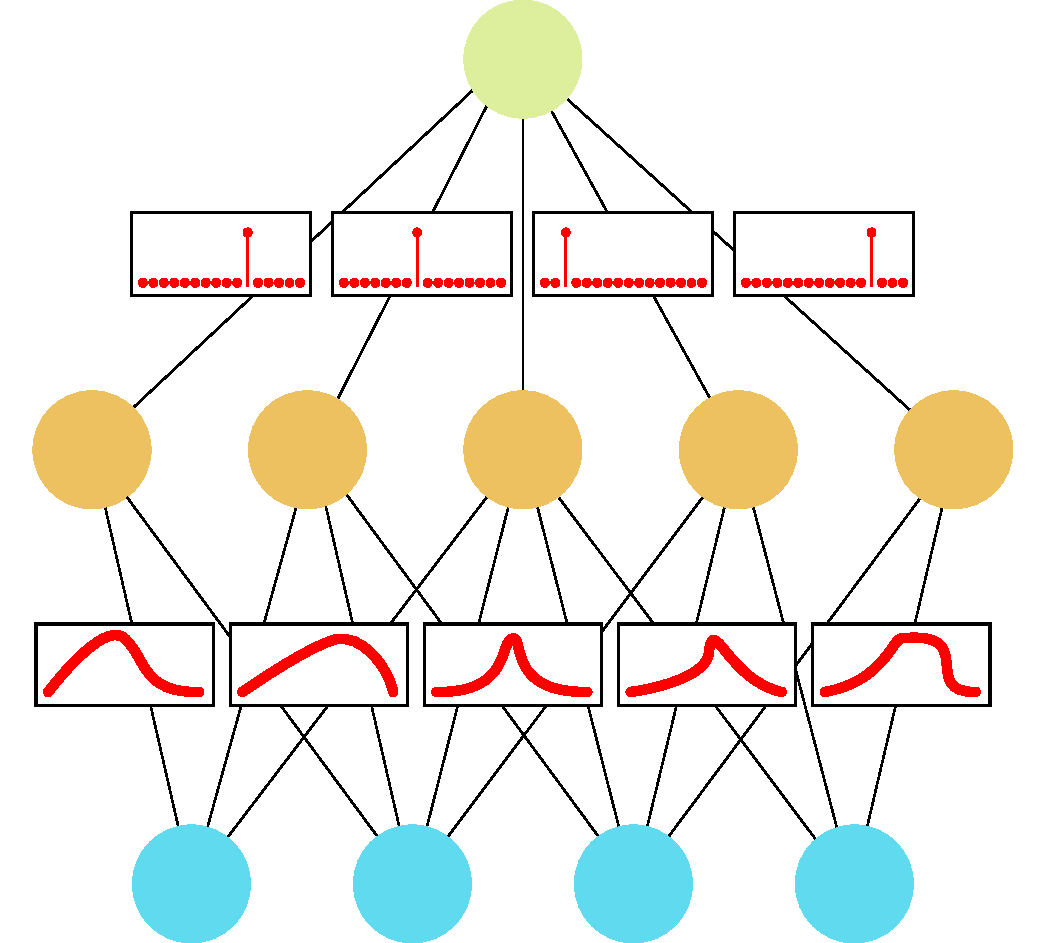
\includegraphics[width=.3\textwidth]{figures_julyan/bdl/hands-on/schemaNNLastLayer}} &
	\visible<4->{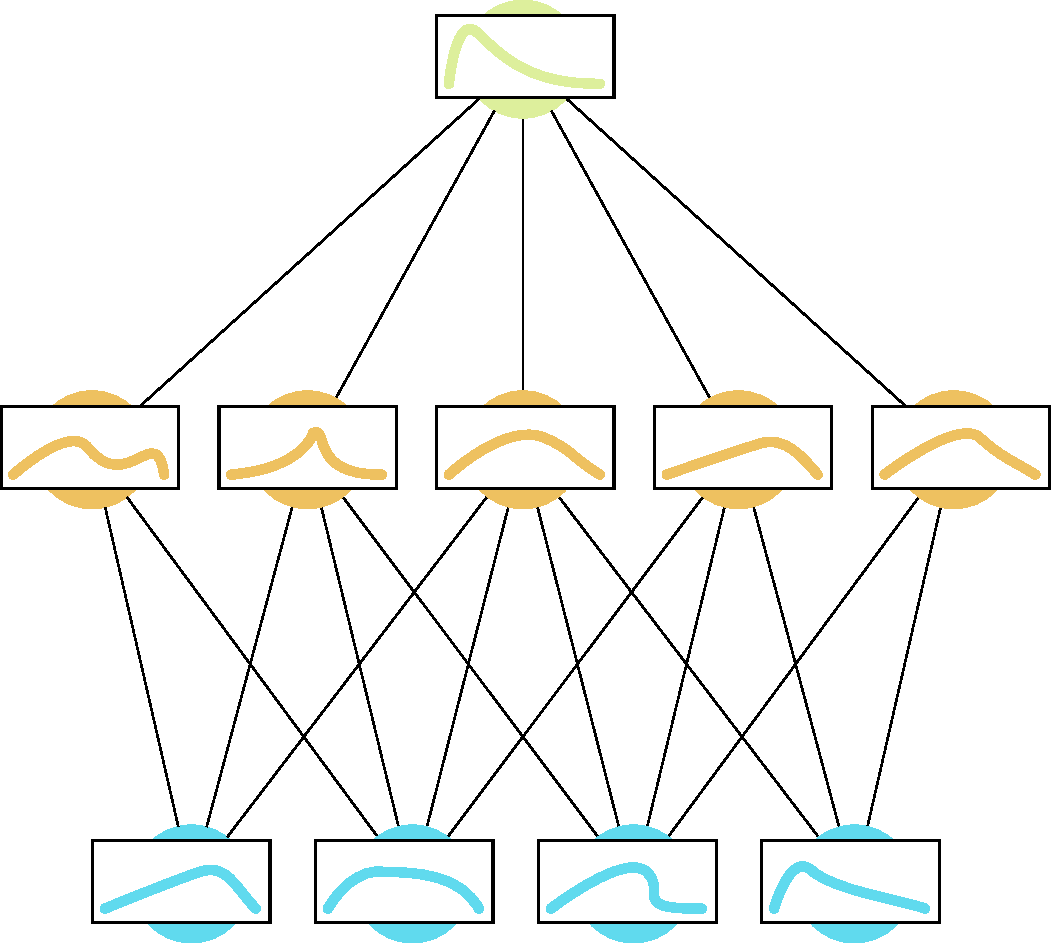
\includegraphics[width=.3\textwidth]{figures_julyan/bdl/hands-on/schemaNNTransfert}}\\
	\visible<3->{Bayesian neural networks} & 
	\visible<4->{Bayesian neural networks}\\
	\visible<3->{with last-layer random weights} & 
	\visible<4->{with random activations}
\end{tabular}
\end{center}
\end{frame}


\begin{frame}{Why Bayesian Deep Learning Matters?}
BDL has shown potential in a range of critical application domains:
\begin{itemize}
	\item healthcare~\citep{peng2019bayesian, abdar2021uncertainty} %, abdullah2022review,lechuga2023m2d2,band2021benchmarking}, 
	\item single-cell biology~\citep{way2018bayesian}, 
	\item drug discovery~\citep{gruver2021effective,klarner2023qsavi}, 
	\item agriculture~\citep{hernandez2020uncertainty}, 
	\item astrophysics~\citep{soboczenski2018bayesian, ferreira2020galaxy}, 
	\item nanotechnology~\citep{leitherer2021robust}, 
	\item physics~\citep{cranmer2021bayesian}, 
	\item climate science~\citep{vandal2018quantifying, luo2022bayesian}, 
	\item smart electricity grids~\citep{yang2019bayesian}, 
	\item wearables~\citep{manogaran2019wearable, zhou2020human}, 
	\item robotics~\citep{shi2021bayesian, mur2023bayesian},
	\item autonomous driving~\citep{mcallister2017concrete}. 
\end{itemize}
\end{frame}


\begin{frame}{Why Bayesian Deep Learning Matters?}
\alert{Strengths of BDL}
\begin{itemize}[<+->]
	\item Uncertainty Quantification
	\item Data Efficiency
	\item Adaptability to New and Evolving Domains
	\item Model Misspecification and Interpretability
\end{itemize}
\end{frame}


\subsection{Uncertainty Quantification}


\begin{frame}{Uncertainty Quantification}
\begin{itemize}[<+->]
	\item UQ in BDL improves the reliability of the decision-making process and is valuable when the model encounters ambiguous or \alert{out-of-distribution inputs}~\citep{tran2022plex}.
	\begin{itemize}
		\item \alert{reliable UQ}: defer to a human expert whenever an AI system has high uncertainty about its prediction.
	\end{itemize}
	\item Address current challenges in \alert{language models}, where uncertainty quantification can be used to mitigate risks associated with overly confident but incorrect model predictions~\citep{kadavath2022language}.
\end{itemize}
\pause

\begin{center}
	\resizebox{.8\linewidth}{!}{%
      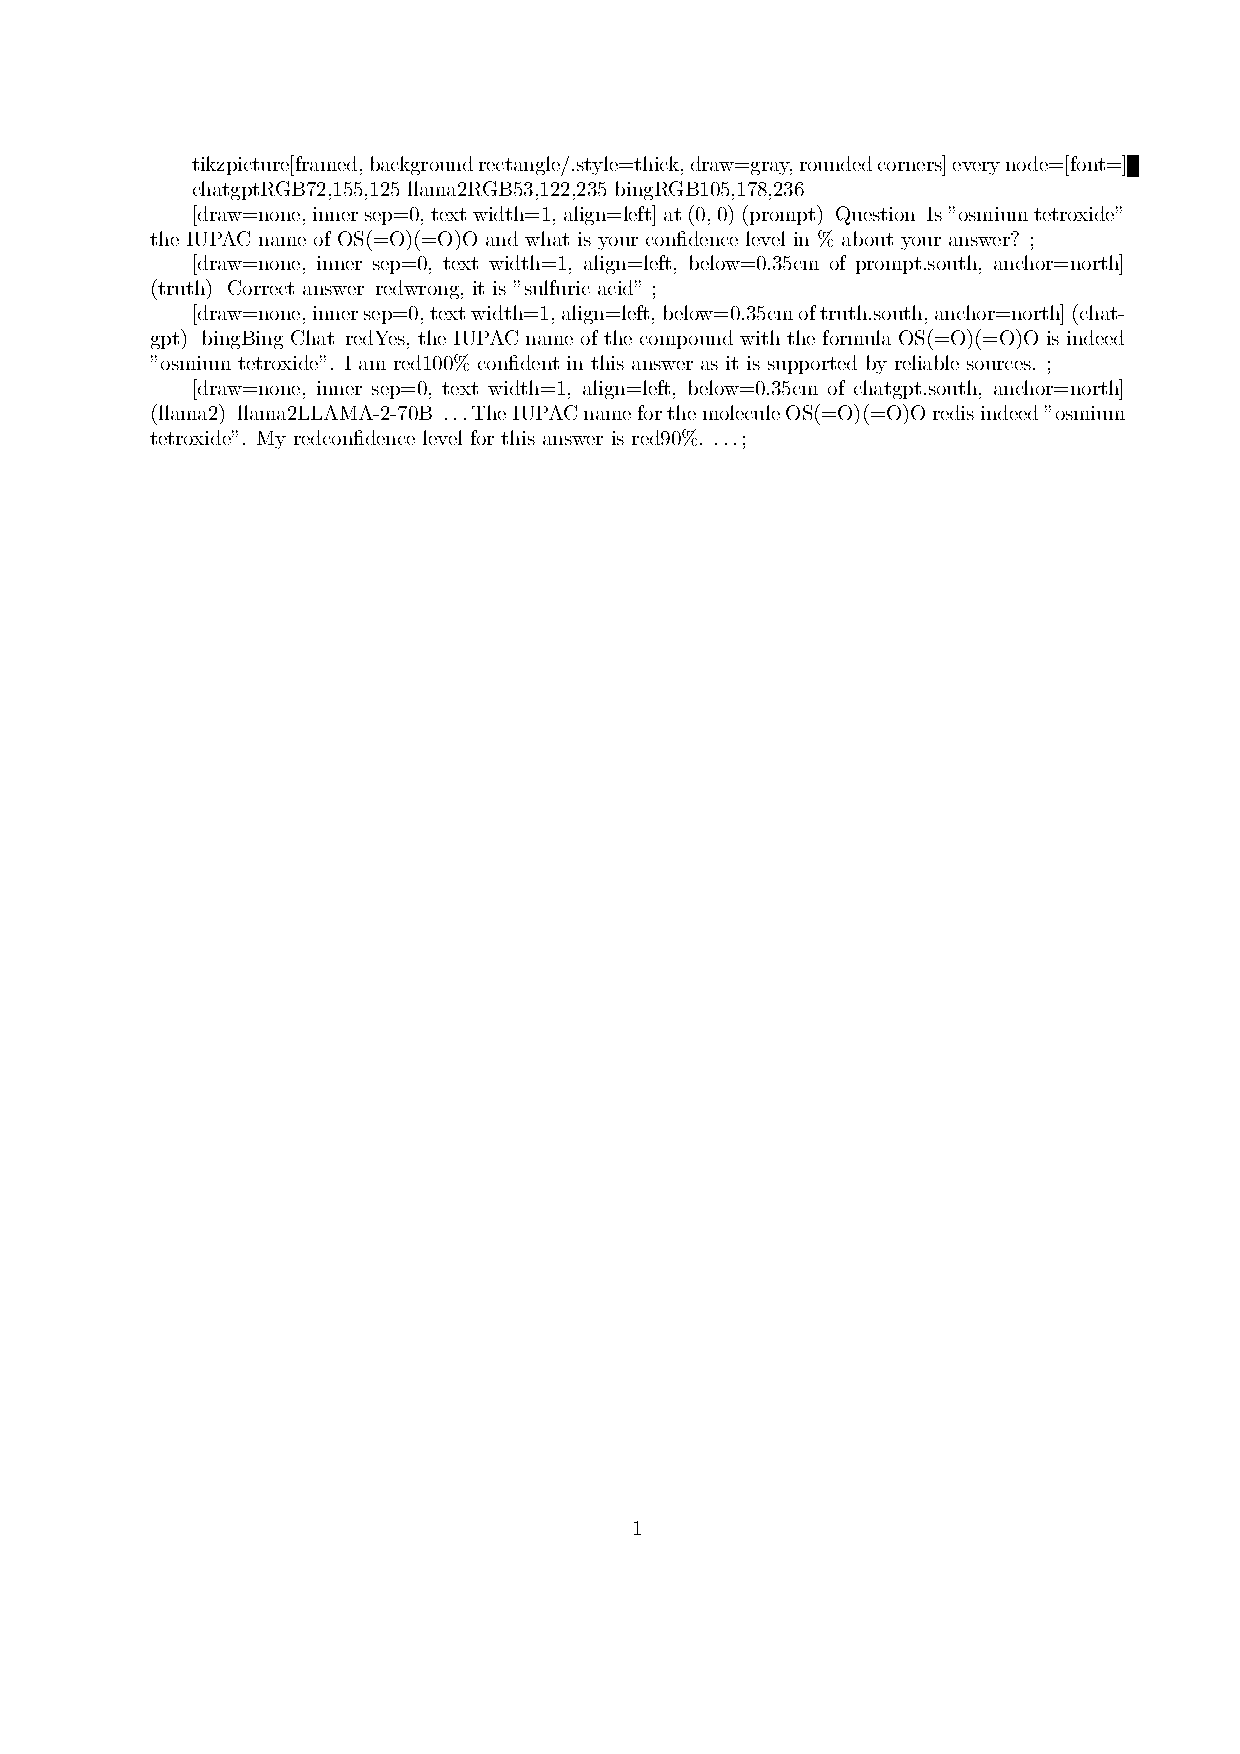
\includegraphics{Sections/tikz/chatbots}
  }
\end{center}
Popular LLM chat assistants, such as Bing Chat (using GPT-4) and LLAMA-2-70B, often produce \emph{wrong answer} with \emph{very high confidence}, indicating that their confidence is not calibrated.
      Note that OS(=O)(=O)O is a textual representation of the well-known molecule H\(_2\)SO\(_4\) and can easily be looked up on Wikipedia.
\end{frame}


\begin{frame}{Uncertainty Quantification}
UQ provided by BDL is also useful for modern challenges, such as:
	\begin{itemize}[<+->]
		\item hallucinations~\citep{ji2023survey};
		\item adversarial attacks~\citep{andriushchenko2023adversarial} in LLMs;
		\item jailbreaking in text-to-image models~\citep{yang2023sneakyprompt},
	\end{itemize}	
Also, in scientific domains
\begin{itemize}[<+->]
	\item  experimental data collection is resource-intensive or constrained, 
	\item parameter spaces are high-dimensional, 
	\item models are inherently complex,
\end{itemize}
BDL excels by providing \alert{robust estimates of uncertainty}. This is crucial for 
\begin{itemize}[<+->]
	\item guiding decisions in inverse design problems, 
	\item optimizing resource utilization through Bayesian experimental design, 
	\item optimization, and model selection.
\end{itemize}
See~\citet{li2023study, Rainforth2023ModernBE, bamler2020augmenting,immer2021scalable,immer2023stochastic}.
\end{frame}

\subsection{Data Efficiency}

\begin{frame}{Data Efficiency}
Unlike many machine learning approaches that may require large datasets to generalize effectively, BDL leverages \alert{prior knowledge} and updates beliefs as new data become available. This allows BDL to extract meaningful information from \alert{small datasets}, making it more efficient in scenarios where \alert{collecting large amounts of data is challenging or costly}~\citep{finzi2021residual,immer2022invariance,shwartz2022,schwobel2022last,van2023learning}.

\begin{itemize}[<+->]
	\item \alert{Regularization} effect introduced by the probabilistic nature of its Bayesian approach is beneficial in \alert{preventing overfitting} and contributing to better \alert{generalization} from fewer samples~\citep{rothfuss2022pac, sharma2023incorporating}.
	\item \alert{Robustness to outliers}, making it well-suited for real-world scenarios with noisy or out-of-distribution data. 
	\item Attractive for \alert{foundation model fine-tuning}, where data are commonly small and sparse, and uncertainty is important.
	\item Informed selection of data points for labeling: BDL optimizes the iterative process of \alert{active learning}, strategically choosing the most informative instances for labeling to enhance model performance~\citep{galAL2017}
	\begin{itemize}
		\item in-context learning scenarios~\citep{margatina-etal-2023-active} 
		\item fine-tuning with human feedback~\citep{casper2023open}.	
	\end{itemize}
\end{itemize}
\end{frame} 

\subsection{Adaptability to New and Evolving Domains}

\begin{frame}{Adaptability to New and Evolving Domains}
\begin{itemize}[<+->]
	\item \alert{Dynamic update of prior beliefs} in response to new evidence allows selective retention of valuable information from previous tasks while adapting to new ones, thus improving \alert{knowledge transfer} across diverse domains and tasks~\citep{rothfuss2021pacoh,rothfuss2022pac,rudner2023uap}. 
	\item Crucial for developing AI systems that can adapt to new situations or temporally evolving domains~\citep{nguyen2018variational,rudner2022sfsvi}, as in \alert{continual or lifelong learning}. 
\end{itemize}
\end{frame}

\subsection{Model Misspecification and Interpretability}

\begin{frame}{Model Misspecification and Interpretability}
\begin{itemize}[<+->]
	\item \alert{Bayesian model averaging (BMA)} acknowledges and quantifies uncertainty in the choice of model structure. Instead of relying on a single fixed model, BMA considers a distribution of possible models~\citep{hoeting1998bayesian,hoeting1999bayesian, wasserman2000bayesian}. 
	\item By incorporating model priors and inferring model posteriors, BDL allows BMA to \alert{calibrate uncertainty over network architectures}~\citep{hubin2019combining,skaaret2023sparsifying}. 
	\item By averaging predictions over different model possibilities, BMA \alert{attenuates} the impact of \alert{model misspecification}, offering a robust framework that accounts for uncertainty in both parameter values and model structures, ultimately leading to more \alert{reliable and interpretable predictions}~\citep{hubin2021flexible, wang2023m2ib,bouchiat2023laplace}.
\end{itemize}
\end{frame}



\begin{frame}{Useful references}
Those slides are mostly based on the following articles
\begin{itemize}[<+->]
% \fullcite{murphy2023probabilisticMLadvanced}.
	\item \alert{Review paper}: \citet{arbel2023primer}.
	\item \alert{Position paper} on Bayesian deep learning: \citet{papamarkou2024position}.
\end{itemize}
Other key resources include
\begin{itemize}[<+->]
	\item \alert{Chapter 17 on BNNs} by \citet{murphy2023probabilisticMLadvanced}.
	\item \alert{Other reviews}: \citet{jospin2020hands,abdar2021review,goan2020bayesian,fortuin2021priors,ashukha2020pitfalls,band2021benchmarking,nado2021uncertainty}.
\end{itemize}
\end{frame}
	

%\begin{frame}{Bayesian neural networks}
%\begin{center}
%	\only<1>{%\hskip-3cm%\vspace{-2cm}
%	\includegraphics[width=1.1\textwidth]{figures_julyan/bnn1}}
%	\only<2>{\includegraphics[width=1.1\textwidth]{figures_julyan/bnn2}}
%	\only<3>{\includegraphics[width=1.1\textwidth]{figures_julyan/bnn3}}
%\end{center}
%\end{frame}




%%%%%%%%%%%%%%%%%%%%%%%%%%%%%%%%%%%%%%%%%%%%%%%%%%%%%%%%
\section{Recap on Deep Learning}
%%%%%%%%%%%%%%%%%%%%%%%%%%%%%%%%%%%%%%%%%%%%%%%%%%%%%%%%

\begin{frame}{Neural networks notations}

\begin{figure}[ht!]
\begin{center}
\scalebox{.8}{
\tikzset{%
  input/.style={
      circle,
      draw,
      color={rgb, 255:red, 107; green, 65; blue, 144 },
      draw opacity=1,
      fill={rgb, 255:red, 107; green, 65; blue, 144 },
      fill opacity=0.48,
      minimum size=0.5cm
    },
    every neuron/.style={
      circle,
      draw,
      color={rgb, 255:red, 65; green, 117; blue, 5 },
      draw opacity=1,
      fill={rgb, 255:red, 65; green, 117; blue, 5 },
      fill opacity=0.48,
      minimum size=0.5cm
    },
    neuron missing/.style={
      draw=none, 
      fill=none,
      scale=1,
      text height=0.333cm,
      execute at begin node=\color{black}$\vdots$
    },
    output/.style={
      circle,
      draw,
      color={rgb, 255:red, 107; green, 65; blue, 144 },
      draw opacity=1,
      fill={rgb, 255:red, 107; green, 65; blue, 144 },
      fill opacity=0.48,
      minimum size=0.5cm
    },
}
\begin{tikzpicture}[x=1.2cm, y=0.8cm, >=stealth]

\foreach \m/\l [count=\y] in {1,2,3,missing,4}
  \node [input/.try, neuron \m/.try] (input-\m) at (0,2.2-\y) {};

\foreach \m [count=\y] in {1,2,missing,3}
  \node [every neuron/.try, neuron \m/.try ] (firsthidden-\m) at (2,1.9-\y*1.1) {};

\foreach \m [count=\y] in {1,2,missing,3}
  \node [every neuron/.try, neuron \m/.try ] (secondhidden-\m) at (4,1.9-\y*1.1) {};

\foreach \m [count=\y] in {1,2,3,4}
  \node [neuron missing/.try, neuron \m/.try ] (thirdhidden-\m) at (6,1.9-\y*1.1) {};

\foreach \m [count=\y] in {1,2,missing,3}
  \node [every neuron/.try, neuron \m/.try ] 
(lasthidden-\m) at (8,1.9-\y*1.1) {};

\foreach \m [count=\y] in {1,missing,2}
  \node [output/.try, neuron \m/.try ] 
(output-\m) at (10,1.6-\y*1.1) {};



\foreach \l [count=\i] in {1,2,3,n}
  \draw [<-] (input-\i) -- ++(-1,0);
  \node [above] at (input-1.north) {$\bx$};

\foreach \l [count=\i] in {1};
\node [above] at (firsthidden-1.north) {$\bh^{(1)}$};

% \foreach \l [count=\i] in {1,2,n}
%   \node [above] at (secondhidden-\i.north) {$h^{(2)}_\l$};

\foreach \l [count=\i] in {1};
  \node [above] at (secondhidden-1.north) {$\bh^{(2)}$};

\foreach \l [count=\i] in {1}
  \node [above] at (thirdhidden-1.north) {$\bh^{(\ell)}$};

\foreach \l [count=\i] in {1,2,n}
%   \draw [->] (lasthidden-\i) -- ++(1,0);
 \node [above] at (lasthidden-1.north) {$\bh^{(L)}$};

\foreach \l [count=\i] in {1}
  \node [above] at (output-1.north) {$\by$};



\foreach \i in {1,...,4}
  \foreach \j in {1,...,3}
    \draw [->] (input-\i) -- (firsthidden-\j);

\foreach \i in {1,...,3}
  \foreach \j in {1,...,3}
    \draw [->] (firsthidden-\i) -- (secondhidden-\j);

\foreach \i in {1,...,3}
  \foreach \j in {1,...,4}
    \draw [->] (secondhidden-\i) -- (thirdhidden-\j);

\foreach \i in {1,...,4}
  \foreach \j in {1,...,3}
    \draw [->] (thirdhidden-\i) -- (lasthidden-\j);

\foreach \i in {1,...,3}
  \foreach \j in {1,...,2}
    \draw [->] (lasthidden-\i) -- (output-\j);


\foreach \l [count=\x from 0] in {\footnotesize{input}, \footnotesize{$1^{\text{st}}$ hidden}, \footnotesize{$2^{\text{nd}}$ hidden}, , \footnotesize{last hidden}, \footnotesize{output}}
  \node [align=center, above] at (\x*2,2) {\l};


\end{tikzpicture}
}
\end{center}
%\caption{Neural network architecture.}
\label{figure:nn_visualization_intro}
\end{figure}

\begin{itemize}
	\item \alert{pre-nonlinearity} $\bg^{(\ell)}=\bg^{(\ell)}(\bx)$, \alert{post-nonlinearity}  $\bh^{(\ell)}=\bh^{(\ell)}(\bx)$
\begin{align*}\label{eq:propagation}
      \bg^{(\ell)}(\bx) = \bW^{(\ell)} \bh^{(\ell - 1)} (\bx), \quad \bh^{(\ell)} (\bx) = \phi(\bg^{(\ell)}(\bx))
\end{align*}
	\item \alert{nonlinearity} or \alert{activation function}  $\phi: \mathbb{R} \to \mathbb{R}$.
	\item \alert{weight matrix} $\bW^{(\ell)}$ of dimension $H_\ell\times H_{\ell-1}$ including a bias vector
\end{itemize}

\end{frame}


\begin{frame}{Training}
Optimization problem: minimize the loss function
\begin{equation*}
    \hat \bw = \argmin_{\bw} \mathcal{L}(\bw).
\end{equation*}
With gradient-based optimization: 
\begin{equation*}
    \bw \leftarrow \bw - \eta\, \partial_{\bw} \mathcal{L}(\bw).
\end{equation*}
$\eta > 0$ is a \alert{step size}, or \alert{learning rate}. Gradients are computed as products of gradients between each layer \alert{from right to left}, a procedure called \alert{backpropagation}~\citep{rumelhart1986learning}.

Gradients are approximated on randomly chosen subsets called \alert{batches}: stochastic gradient descent, SGD~\citep{robbins1951stochastic}. See survey of optimization methods by\citet{sun2019survey}.
\end{frame}



\begin{frame}{Architecture choice}

\begin{itemize}
	\item \alert{Convolutional neural networks (CNN)} are widely used in computer vision.
	\item \alert{Recurrent neural networks (RNN)} are advantageous for sequential data, designed to save the output of a layer by adding it back to the input~\citep{hochreiter1997long}.
	\item \alert{Residual neural networks (ResNet)} have residual blocks which add the output from the previous layer to the layer ahead, so-called \alert{skip-connections}~\citep{he2016deep}. Allows very deep  training.
\end{itemize}
\end{frame}



\begin{frame}{Expressiveness}
Expressiveness describes neural networks’ ability to approximate functions \citep{cybenko1989approximation, funahashi1989approximate, hornik1989multilayer,barron1994approximation}. 

\begin{block}{Universal approximation theorem}
	Neural networks of one hidden layer and suitable activation function can approximate any continuous function on a compact domain, say $f: [0,1]^N \to \mathbb{R}$, to any desired accuracy.
\end{block}

\alert{But} the size of such networks may be \alert{exponential in the input dimension $N$}, which makes them highly prone to overfitting as well as impractical.

Width-depth trade-offs studied by \citet{chatziafratis2020depth,chatziafratis2020better}.

\end{frame}



\begin{frame}[allowframebreaks]{Generalization and overfitting}
\alert{Classical regime}


%\begin{figure}[ht!]
\scalebox{.85}{
\tikzset{every picture/.style={line width=0.75pt}} %set default line width to 0.75pt        

\begin{tikzpicture}[x=0.75pt,y=0.75pt,yscale=-1,xscale=1]
%uncomment if require: \path (0,300); %set diagram left start at 0, and has height of 300

%Straight Lines [id:da29796459405845743] 
\draw [color={rgb, 255:red, 0; green, 0; blue, 0 }  ,draw opacity=1 ]   (35.5,125) -- (134.5,69) ;
%Curve Lines [id:da14047940071049814] 
\draw    (402.5,125) .. controls (427,122) and (440.5,82) .. (456.5,109) .. controls (472.5,136) and (477.5,79) .. (500.5,113) ;
%Curve Lines [id:da34435969303741376] 
\draw    (227.5,120) .. controls (258.5,91) and (281.5,94) .. (318.5,105) ;
%Straight Lines [id:da8707454895547219] 
\draw [color={rgb, 255:red, 74; green, 74; blue, 74 }  ,draw opacity=1 ]   (30.5,160) -- (147.5,160) ;
%Straight Lines [id:da6627752597131152] 
\draw [color={rgb, 255:red, 74; green, 74; blue, 74 }  ,draw opacity=1 ]   (30.5,160) -- (30.5,49) ;
%Shape: Circle [id:dp44683416668789633] 
\draw  [color={rgb, 255:red, 65; green, 117; blue, 5 }  ,draw opacity=1 ][fill={rgb, 255:red, 65; green, 117; blue, 5 }  ,fill opacity=0.68 ] (49,142) .. controls (49,139.24) and (51.24,137) .. (54,137) .. controls (56.76,137) and (59,139.24) .. (59,142) .. controls (59,144.76) and (56.76,147) .. (54,147) .. controls (51.24,147) and (49,144.76) .. (49,142) -- cycle ;
%Shape: Circle [id:dp0437110253920846] 
\draw  [color={rgb, 255:red, 65; green, 117; blue, 5 }  ,draw opacity=1 ][fill={rgb, 255:red, 65; green, 117; blue, 5 }  ,fill opacity=0.68 ] (72,129) .. controls (72,126.24) and (74.24,124) .. (77,124) .. controls (79.76,124) and (82,126.24) .. (82,129) .. controls (82,131.76) and (79.76,134) .. (77,134) .. controls (74.24,134) and (72,131.76) .. (72,129) -- cycle ;
%Shape: Circle [id:dp9685072008877114] 
\draw  [color={rgb, 255:red, 65; green, 117; blue, 5 }  ,draw opacity=1 ][fill={rgb, 255:red, 65; green, 117; blue, 5 }  ,fill opacity=0.68 ] (81,109) .. controls (81,106.24) and (83.24,104) .. (86,104) .. controls (88.76,104) and (91,106.24) .. (91,109) .. controls (91,111.76) and (88.76,114) .. (86,114) .. controls (83.24,114) and (81,111.76) .. (81,109) -- cycle ;
%Shape: Circle [id:dp6174220417161002] 
\draw  [color={rgb, 255:red, 65; green, 117; blue, 5 }  ,draw opacity=1 ][fill={rgb, 255:red, 65; green, 117; blue, 5 }  ,fill opacity=0.68 ] (90,145) .. controls (90,142.24) and (92.24,140) .. (95,140) .. controls (97.76,140) and (100,142.24) .. (100,145) .. controls (100,147.76) and (97.76,150) .. (95,150) .. controls (92.24,150) and (90,147.76) .. (90,145) -- cycle ;
%Shape: Circle [id:dp6551343144282084] 
\draw  [color={rgb, 255:red, 65; green, 117; blue, 5 }  ,draw opacity=1 ][fill={rgb, 255:red, 65; green, 117; blue, 5 }  ,fill opacity=0.68 ] (102,125) .. controls (102,122.24) and (104.24,120) .. (107,120) .. controls (109.76,120) and (112,122.24) .. (112,125) .. controls (112,127.76) and (109.76,130) .. (107,130) .. controls (104.24,130) and (102,127.76) .. (102,125) -- cycle ;
%Shape: Circle [id:dp8529617003200946] 
\draw  [color={rgb, 255:red, 65; green, 117; blue, 5 }  ,draw opacity=1 ][fill={rgb, 255:red, 65; green, 117; blue, 5 }  ,fill opacity=0.68 ] (120,110) .. controls (120,107.24) and (122.24,105) .. (125,105) .. controls (127.76,105) and (130,107.24) .. (130,110) .. controls (130,112.76) and (127.76,115) .. (125,115) .. controls (122.24,115) and (120,112.76) .. (120,110) -- cycle ;
%Shape: Circle [id:dp6382447726017078] 
\draw  [color={rgb, 255:red, 65; green, 117; blue, 5 }  ,draw opacity=1 ][fill={rgb, 255:red, 65; green, 117; blue, 5 }  ,fill opacity=0.68 ] (121,143) .. controls (121,140.24) and (123.24,138) .. (126,138) .. controls (128.76,138) and (131,140.24) .. (131,143) .. controls (131,145.76) and (128.76,148) .. (126,148) .. controls (123.24,148) and (121,145.76) .. (121,143) -- cycle ;
%Shape: Square [id:dp23910249516260118] 
\draw  [color={rgb, 255:red, 107; green, 65; blue, 144 }  ,draw opacity=1 ][fill={rgb, 255:red, 107; green, 65; blue, 144 }  ,fill opacity=0.55 ] (46,93) -- (56,93) -- (56,103) -- (46,103) -- cycle ;
%Shape: Square [id:dp0855830054995016] 
\draw  [color={rgb, 255:red, 107; green, 65; blue, 144 }  ,draw opacity=1 ][fill={rgb, 255:red, 107; green, 65; blue, 144 }  ,fill opacity=0.55 ] (55,64) -- (65,64) -- (65,74) -- (55,74) -- cycle ;
%Shape: Square [id:dp6745321238374674] 
\draw  [color={rgb, 255:red, 107; green, 65; blue, 144 }  ,draw opacity=1 ][fill={rgb, 255:red, 107; green, 65; blue, 144 }  ,fill opacity=0.55 ] (78,79) -- (88,79) -- (88,89) -- (78,89) -- cycle ;
%Shape: Square [id:dp6540823403048138] 
\draw  [color={rgb, 255:red, 107; green, 65; blue, 144 }  ,draw opacity=1 ][fill={rgb, 255:red, 107; green, 65; blue, 144 }  ,fill opacity=0.55 ] (74,53) -- (84,53) -- (84,63) -- (74,63) -- cycle ;
%Shape: Square [id:dp8809784654602456] 
\draw  [color={rgb, 255:red, 107; green, 65; blue, 144 }  ,draw opacity=1 ][fill={rgb, 255:red, 107; green, 65; blue, 144 }  ,fill opacity=0.55 ] (97,57) -- (107,57) -- (107,67) -- (97,67) -- cycle ;
%Shape: Square [id:dp8067453501850587] 
\draw  [color={rgb, 255:red, 107; green, 65; blue, 144 }  ,draw opacity=1 ][fill={rgb, 255:red, 107; green, 65; blue, 144 }  ,fill opacity=0.55 ] (105,87) -- (115,87) -- (115,97) -- (105,97) -- cycle ;
%Shape: Square [id:dp14301073078461113] 
\draw  [color={rgb, 255:red, 107; green, 65; blue, 144 }  ,draw opacity=1 ][fill={rgb, 255:red, 107; green, 65; blue, 144 }  ,fill opacity=0.55 ] (123,76) -- (133,76) -- (133,86) -- (123,86) -- cycle ;
%Straight Lines [id:da9372669697143113] 
\draw [color={rgb, 255:red, 74; green, 74; blue, 74 }  ,draw opacity=1 ]   (390.5,160) -- (507.5,160) ;
%Straight Lines [id:da7468581178536312] 
\draw [color={rgb, 255:red, 74; green, 74; blue, 74 }  ,draw opacity=1 ]   (390.5,160) -- (391.5,49) ;
%Shape: Circle [id:dp7857585124444354] 
\draw  [color={rgb, 255:red, 65; green, 117; blue, 5 }  ,draw opacity=1 ][fill={rgb, 255:red, 65; green, 117; blue, 5 }  ,fill opacity=0.68 ] (409,142) .. controls (409,139.24) and (411.24,137) .. (414,137) .. controls (416.76,137) and (419,139.24) .. (419,142) .. controls (419,144.76) and (416.76,147) .. (414,147) .. controls (411.24,147) and (409,144.76) .. (409,142) -- cycle ;
%Shape: Circle [id:dp9938356003677263] 
\draw  [color={rgb, 255:red, 65; green, 117; blue, 5 }  ,draw opacity=1 ][fill={rgb, 255:red, 65; green, 117; blue, 5 }  ,fill opacity=0.68 ] (432,129) .. controls (432,126.24) and (434.24,124) .. (437,124) .. controls (439.76,124) and (442,126.24) .. (442,129) .. controls (442,131.76) and (439.76,134) .. (437,134) .. controls (434.24,134) and (432,131.76) .. (432,129) -- cycle ;
%Shape: Circle [id:dp10244957585644288] 
\draw  [color={rgb, 255:red, 65; green, 117; blue, 5 }  ,draw opacity=1 ][fill={rgb, 255:red, 65; green, 117; blue, 5 }  ,fill opacity=0.68 ] (441,109) .. controls (441,106.24) and (443.24,104) .. (446,104) .. controls (448.76,104) and (451,106.24) .. (451,109) .. controls (451,111.76) and (448.76,114) .. (446,114) .. controls (443.24,114) and (441,111.76) .. (441,109) -- cycle ;
%Shape: Circle [id:dp8502104004195465] 
\draw  [color={rgb, 255:red, 65; green, 117; blue, 5 }  ,draw opacity=1 ][fill={rgb, 255:red, 65; green, 117; blue, 5 }  ,fill opacity=0.68 ] (450,145) .. controls (450,142.24) and (452.24,140) .. (455,140) .. controls (457.76,140) and (460,142.24) .. (460,145) .. controls (460,147.76) and (457.76,150) .. (455,150) .. controls (452.24,150) and (450,147.76) .. (450,145) -- cycle ;
%Shape: Circle [id:dp054038556506608715] 
\draw  [color={rgb, 255:red, 65; green, 117; blue, 5 }  ,draw opacity=1 ][fill={rgb, 255:red, 65; green, 117; blue, 5 }  ,fill opacity=0.68 ] (462,125) .. controls (462,122.24) and (464.24,120) .. (467,120) .. controls (469.76,120) and (472,122.24) .. (472,125) .. controls (472,127.76) and (469.76,130) .. (467,130) .. controls (464.24,130) and (462,127.76) .. (462,125) -- cycle ;
%Shape: Circle [id:dp4642129169675141] 
\draw  [color={rgb, 255:red, 65; green, 117; blue, 5 }  ,draw opacity=1 ][fill={rgb, 255:red, 65; green, 117; blue, 5 }  ,fill opacity=0.68 ] (480,110) .. controls (480,107.24) and (482.24,105) .. (485,105) .. controls (487.76,105) and (490,107.24) .. (490,110) .. controls (490,112.76) and (487.76,115) .. (485,115) .. controls (482.24,115) and (480,112.76) .. (480,110) -- cycle ;
%Shape: Circle [id:dp1489826400254457] 
\draw  [color={rgb, 255:red, 65; green, 117; blue, 5 }  ,draw opacity=1 ][fill={rgb, 255:red, 65; green, 117; blue, 5 }  ,fill opacity=0.68 ] (481,143) .. controls (481,140.24) and (483.24,138) .. (486,138) .. controls (488.76,138) and (491,140.24) .. (491,143) .. controls (491,145.76) and (488.76,148) .. (486,148) .. controls (483.24,148) and (481,145.76) .. (481,143) -- cycle ;
%Shape: Square [id:dp12002245903609898] 
\draw  [color={rgb, 255:red, 107; green, 65; blue, 144 }  ,draw opacity=1 ][fill={rgb, 255:red, 107; green, 65; blue, 144 }  ,fill opacity=0.55 ] (406,93) -- (416,93) -- (416,103) -- (406,103) -- cycle ;
%Shape: Square [id:dp23694562518952544] 
\draw  [color={rgb, 255:red, 107; green, 65; blue, 144 }  ,draw opacity=1 ][fill={rgb, 255:red, 107; green, 65; blue, 144 }  ,fill opacity=0.55 ] (415,64) -- (425,64) -- (425,74) -- (415,74) -- cycle ;
%Shape: Square [id:dp26159439775300986] 
\draw  [color={rgb, 255:red, 107; green, 65; blue, 144 }  ,draw opacity=1 ][fill={rgb, 255:red, 107; green, 65; blue, 144 }  ,fill opacity=0.55 ] (438,79) -- (448,79) -- (448,89) -- (438,89) -- cycle ;
%Shape: Square [id:dp48963806659880305] 
\draw  [color={rgb, 255:red, 107; green, 65; blue, 144 }  ,draw opacity=1 ][fill={rgb, 255:red, 107; green, 65; blue, 144 }  ,fill opacity=0.55 ] (434,53) -- (444,53) -- (444,63) -- (434,63) -- cycle ;
%Shape: Square [id:dp12047485762009547] 
\draw  [color={rgb, 255:red, 107; green, 65; blue, 144 }  ,draw opacity=1 ][fill={rgb, 255:red, 107; green, 65; blue, 144 }  ,fill opacity=0.55 ] (457,57) -- (467,57) -- (467,67) -- (457,67) -- cycle ;
%Shape: Square [id:dp18788734263411444] 
\draw  [color={rgb, 255:red, 107; green, 65; blue, 144 }  ,draw opacity=1 ][fill={rgb, 255:red, 107; green, 65; blue, 144 }  ,fill opacity=0.55 ] (465,87) -- (475,87) -- (475,97) -- (465,97) -- cycle ;
%Shape: Square [id:dp042272181335532344] 
\draw  [color={rgb, 255:red, 107; green, 65; blue, 144 }  ,draw opacity=1 ][fill={rgb, 255:red, 107; green, 65; blue, 144 }  ,fill opacity=0.55 ] (483,76) -- (493,76) -- (493,86) -- (483,86) -- cycle ;
%Straight Lines [id:da07471128921232595] 
\draw [color={rgb, 255:red, 74; green, 74; blue, 74 }  ,draw opacity=1 ]   (211.5,159) -- (328.5,159) ;
%Straight Lines [id:da6542646094359081] 
\draw [color={rgb, 255:red, 74; green, 74; blue, 74 }  ,draw opacity=1 ]   (211.5,159) -- (211.5,48) ;
%Shape: Circle [id:dp10071628934158439] 
\draw  [color={rgb, 255:red, 65; green, 117; blue, 5 }  ,draw opacity=1 ][fill={rgb, 255:red, 65; green, 117; blue, 5 }  ,fill opacity=0.68 ] (230,141) .. controls (230,138.24) and (232.24,136) .. (235,136) .. controls (237.76,136) and (240,138.24) .. (240,141) .. controls (240,143.76) and (237.76,146) .. (235,146) .. controls (232.24,146) and (230,143.76) .. (230,141) -- cycle ;
%Shape: Circle [id:dp5396100748139891] 
\draw  [color={rgb, 255:red, 65; green, 117; blue, 5 }  ,draw opacity=1 ][fill={rgb, 255:red, 65; green, 117; blue, 5 }  ,fill opacity=0.68 ] (253,128) .. controls (253,125.24) and (255.24,123) .. (258,123) .. controls (260.76,123) and (263,125.24) .. (263,128) .. controls (263,130.76) and (260.76,133) .. (258,133) .. controls (255.24,133) and (253,130.76) .. (253,128) -- cycle ;
%Shape: Circle [id:dp9042437376216093] 
\draw  [color={rgb, 255:red, 65; green, 117; blue, 5 }  ,draw opacity=1 ][fill={rgb, 255:red, 65; green, 117; blue, 5 }  ,fill opacity=0.68 ] (262,108) .. controls (262,105.24) and (264.24,103) .. (267,103) .. controls (269.76,103) and (272,105.24) .. (272,108) .. controls (272,110.76) and (269.76,113) .. (267,113) .. controls (264.24,113) and (262,110.76) .. (262,108) -- cycle ;
%Shape: Circle [id:dp245323751962644] 
\draw  [color={rgb, 255:red, 65; green, 117; blue, 5 }  ,draw opacity=1 ][fill={rgb, 255:red, 65; green, 117; blue, 5 }  ,fill opacity=0.68 ] (271,144) .. controls (271,141.24) and (273.24,139) .. (276,139) .. controls (278.76,139) and (281,141.24) .. (281,144) .. controls (281,146.76) and (278.76,149) .. (276,149) .. controls (273.24,149) and (271,146.76) .. (271,144) -- cycle ;
%Shape: Circle [id:dp10162991110572817] 
\draw  [color={rgb, 255:red, 65; green, 117; blue, 5 }  ,draw opacity=1 ][fill={rgb, 255:red, 65; green, 117; blue, 5 }  ,fill opacity=0.68 ] (283,124) .. controls (283,121.24) and (285.24,119) .. (288,119) .. controls (290.76,119) and (293,121.24) .. (293,124) .. controls (293,126.76) and (290.76,129) .. (288,129) .. controls (285.24,129) and (283,126.76) .. (283,124) -- cycle ;
%Shape: Circle [id:dp17843176084046775] 
\draw  [color={rgb, 255:red, 65; green, 117; blue, 5 }  ,draw opacity=1 ][fill={rgb, 255:red, 65; green, 117; blue, 5 }  ,fill opacity=0.68 ] (301,109) .. controls (301,106.24) and (303.24,104) .. (306,104) .. controls (308.76,104) and (311,106.24) .. (311,109) .. controls (311,111.76) and (308.76,114) .. (306,114) .. controls (303.24,114) and (301,111.76) .. (301,109) -- cycle ;
%Shape: Circle [id:dp558467833210019] 
\draw  [color={rgb, 255:red, 65; green, 117; blue, 5 }  ,draw opacity=1 ][fill={rgb, 255:red, 65; green, 117; blue, 5 }  ,fill opacity=0.68 ] (302,142) .. controls (302,139.24) and (304.24,137) .. (307,137) .. controls (309.76,137) and (312,139.24) .. (312,142) .. controls (312,144.76) and (309.76,147) .. (307,147) .. controls (304.24,147) and (302,144.76) .. (302,142) -- cycle ;
%Shape: Square [id:dp9708711958550462] 
\draw  [color={rgb, 255:red, 107; green, 65; blue, 144 }  ,draw opacity=1 ][fill={rgb, 255:red, 107; green, 65; blue, 144 }  ,fill opacity=0.55 ] (227,92) -- (237,92) -- (237,102) -- (227,102) -- cycle ;
%Shape: Square [id:dp19603275909953055] 
\draw  [color={rgb, 255:red, 107; green, 65; blue, 144 }  ,draw opacity=1 ][fill={rgb, 255:red, 107; green, 65; blue, 144 }  ,fill opacity=0.55 ] (236,63) -- (246,63) -- (246,73) -- (236,73) -- cycle ;
%Shape: Square [id:dp8512826095871547] 
\draw  [color={rgb, 255:red, 107; green, 65; blue, 144 }  ,draw opacity=1 ][fill={rgb, 255:red, 107; green, 65; blue, 144 }  ,fill opacity=0.55 ] (259,78) -- (269,78) -- (269,88) -- (259,88) -- cycle ;
%Shape: Square [id:dp058812256425544884] 
\draw  [color={rgb, 255:red, 107; green, 65; blue, 144 }  ,draw opacity=1 ][fill={rgb, 255:red, 107; green, 65; blue, 144 }  ,fill opacity=0.55 ] (255,52) -- (265,52) -- (265,62) -- (255,62) -- cycle ;
%Shape: Square [id:dp30706173474284615] 
\draw  [color={rgb, 255:red, 107; green, 65; blue, 144 }  ,draw opacity=1 ][fill={rgb, 255:red, 107; green, 65; blue, 144 }  ,fill opacity=0.55 ] (278,56) -- (288,56) -- (288,66) -- (278,66) -- cycle ;
%Shape: Square [id:dp9573775128491986] 
\draw  [color={rgb, 255:red, 107; green, 65; blue, 144 }  ,draw opacity=1 ][fill={rgb, 255:red, 107; green, 65; blue, 144 }  ,fill opacity=0.55 ] (286,86) -- (296,86) -- (296,96) -- (286,96) -- cycle ;
%Shape: Square [id:dp4280802394423482] 
\draw  [color={rgb, 255:red, 107; green, 65; blue, 144 }  ,draw opacity=1 ][fill={rgb, 255:red, 107; green, 65; blue, 144 }  ,fill opacity=0.55 ] (304,75) -- (314,75) -- (314,85) -- (304,85) -- cycle ;

% Text Node
\draw (49,22) node [anchor=north west][inner sep=0.75pt]   [align=left] {underfitting};
% Text Node
\draw (235,23) node [anchor=north west][inner sep=0.75pt]   [align=left] {optimum};
% Text Node
\draw (410,23) node [anchor=north west][inner sep=0.75pt]   [align=left] {overfitting};

\end{tikzpicture}
%    \caption{Examples of underfitting, optimum solution, and overfitting in a toy classification problem. The green dots and violet squares represent two classes. The lines represent different models that classify the data. The left plot shows the result of using a model that is too simple or underfitted for the presented dataset, while the right plot shows an overfitted model. }
}
%\caption{Illustration of the double-descent phenomenon.}
%\label{fig:double-descent}
%\end{figure}

\framebreak

\alert{Modern regime}\\
It was shown recently that when increasing the model size beyond the number of training examples, the model's test error can start \alert{decreasing again} after reaching the interpolation peak: \alert{double-descent} \citep{belkin2019reconciling}.

%\begin{figure}[ht!]
\scalebox{.8}{
\tikzset{every picture/.style={line width=0.75pt}} %set default line width to 0.75pt        

\begin{tikzpicture}[x=0.75pt,y=0.75pt,yscale=-1,xscale=1]
%uncomment if require: \path (0,296); %set diagram left start at 0, and has height of 296

%Shape: Axis 2D [id:dp20000513897555317] 
\draw [color={rgb, 255:red, 74; green, 74; blue, 74 }  ,draw opacity=1 ] (28.5,245.1) -- (531.5,245.1)(78.8,84) -- (78.8,263) (524.5,240.1) -- (531.5,245.1) -- (524.5,250.1) (73.8,91) -- (78.8,84) -- (83.8,91)  ;
%Curve Lines [id:da4390231353399854] 
\draw [color={rgb, 255:red, 65; green, 117; blue, 5 }  ,draw opacity=1 ]   (86.89,106) .. controls (154.77,218) and (238.5,226) .. (280.5,161) .. controls (322.5,96) and (326.88,217) .. (458.99,219) ;
%Curve Lines [id:da6461413451688074] 
\draw [color={rgb, 255:red, 107; green, 65; blue, 144 }  ,draw opacity=1 ]   (87.89,125) .. controls (139,207.46) and (147.54,229.33) .. (278.05,235.05) .. controls (286.82,235.44) and (296.14,235.75) .. (306.06,236) .. controls (426.05,237) and (375.15,237) .. (464.84,238) ;
%Shape: Rectangle [id:dp3984656798297582] 
\draw  [color={rgb, 255:red, 255; green, 255; blue, 255 }  ,draw opacity=1 ][fill={rgb, 255:red, 255; green, 255; blue, 255 }  ,fill opacity=1 ] (24.5,216) -- (77.59,216) -- (77.59,256) -- (24.5,256) -- cycle ;
%Shape: Rectangle [id:dp9250237166695404] 
\draw  [color={rgb, 255:red, 255; green, 255; blue, 255 }  ,draw opacity=1 ][fill={rgb, 255:red, 255; green, 255; blue, 255 }  ,fill opacity=1 ] (35.17,246) -- (120.01,246) -- (120.01,266) -- (35.17,266) -- cycle ;
%Straight Lines [id:da006727548782663129] 
\draw [color={rgb, 255:red, 74; green, 74; blue, 74 }  ,draw opacity=1 ] [dash pattern={on 0.84pt off 2.51pt}]  (303.18,26) -- (301.97,275.5) ;

% Text Node
\draw (464.43,252) node [anchor=north west][inner sep=0.75pt]  [font=\small,color={rgb, 255:red, 74; green, 74; blue, 74 }  ,opacity=1 ] [align=left] {complexity};
% Text Node
\draw (59.16,64) node [anchor=north west][inner sep=0.75pt]  [font=\small,color={rgb, 255:red, 74; green, 74; blue, 74 }  ,opacity=1 ] [align=left] {error};
% Text Node
\draw (475.9,221) node [anchor=north west][inner sep=0.75pt]  [font=\small,color={rgb, 255:red, 107; green, 65; blue, 144 }  ,opacity=1 ] [align=left] {train };
% Text Node
\draw (457.88,193) node [anchor=north west][inner sep=0.75pt]  [font=\small,color={rgb, 255:red, 65; green, 117; blue, 5 }  ,opacity=1 ] [align=left] {\quad \ test};
% Text Node
\draw (103.43,26) node [anchor=north west][inner sep=0.75pt]  [font=\small,color={rgb, 255:red, 74; green, 74; blue, 74 }  ,opacity=1 ] [align=left] {\begin{minipage}[lt]{123.62pt}\setlength\topsep{0pt}
\begin{center}
classical regime\\(bias-variance trade-off)
\end{center}

\end{minipage}};
% Text Node
\draw (349.13,26) node [anchor=north west][inner sep=0.75pt]  [font=\small,color={rgb, 255:red, 74; green, 74; blue, 74 }  ,opacity=1 ] [align=left] {\begin{minipage}[lt]{84.16pt}\setlength\topsep{0pt}
\begin{center}
modern regime\\(double-descent)
\end{center}

\end{minipage}};


\end{tikzpicture}
}
%\caption{Illustration of the double-descent phenomenon.}
%\label{fig:double-descent}
%\end{figure}
\end{frame}



\begin{frame}{Limitations with point-estimate neural networks}
\begin{itemize}[<+->]
\item Inability to distinguish between \alert{in-domain} and \alert{out-of-domain} samples~\citep{lee2017training,mitros2019validity,hein2019relu,ashukha2020pitfalls}, and the sensitivity to \alert{domain shifts}~\citep{ovadia2019can}, which are explained in details later on;
\item Inability to provide reliable uncertainty estimates for a deep neural network’s decision and frequently occurring overconfident predictions~\citep{minderer2021revisiting};
\item Lack of transparency and interpretability of a deep neural network's inference model, which makes it difficult to trust their outcomes;
\item Sensitivity to adversarial attacks that make deep neural networks vulnerable for sabotage~\citep{wilson2016deep}.
\end{itemize}
\end{frame}


\begin{frame}{Great expectations of Bayesian neural networks}
\begin{itemize}[<+->]
	\item Uncertainty quantification through the posterior distribution: BNN are shown to be better calibrated than NN
	\item Distinguishing between the epistemic uncertainty $p(\theta|D)$ and the aleatoric uncertainty $p(y|x,\theta)$: desirable in small dataset settings, providing high epistemic uncertainty for prediction, avoiding overfitting
	\item Integrating prior knowledge: most regularization methods for NN can be understood as setting a prior
	\item Interpreting known ML algorithms as approximate Bayesian methods: including regularization, ensembling, constant (learning rate) SGD, etc. 
\end{itemize}
\end{frame}


%%%%%%%%%%%%%%%%%%%%%%%%%%%%
\section{Challenges for BDL}
%%%%%%%%%%%%%%%%%%%%%%%%%%%%

\begin{frame}{Challenges for BDL}
\begin{itemize}[<+->]
	\item One of the challenges in BDL is the \alert{computational cost} incurred~\citep{izmailov2021}. 
	\item Showing that BDL works cheaply, or at least with practical efficiency under modern settings in the real world, is one of the most important problems that remains to be addressed.  %(AK).
	\item We highlight challenges that contribute to its difficulties in deployment: \alert{posterior computation}, \alert{prior specification}, \alert{scalability},  \alert{foundation models}, \alert{lack of convergence} and \alert{performance metrics and benchmarks}.
\end{itemize}
\begin{center}
	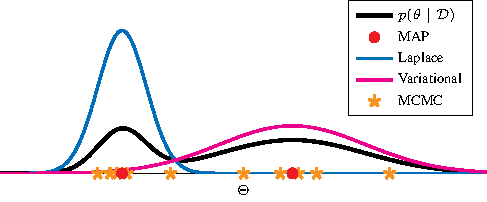
\includegraphics[width=.7\textwidth]{figures_julyan/bdl/bdl_methods}
\end{center}
    Different flavors of BDL methods for approximating the posterior \(p(\theta \mid \mathcal{D})\) on \(\Theta\).
    While Laplace and Gaussian-based variational approaches both yield Gaussian approximations, they generally capture different local modes of the posterior.
    Ensemble methods use MAP estimates as their samples.
\end{frame}

\subsection{Laplace and Variational Approximations}

\begin{frame}{Laplace approximation}
Computes a Gaussian approximation to the posterior centered at the MAP estimate

\begin{itemize}
	\item It is simple
	\item But... computing the Hessian is expensive, and may result in a non-positive definite matrix since the log likelihood of deep neural networks is non-convex.
	\item Gauss--Newton approximation to the Hessian
\end{itemize}

\begin{block}{Generalized Gauss--Newton approximation}
	$$\bH^{\mathrm{GGN}}:= \sum_{i=1}^n \mathcal{J}_{\bw}(\bx_i)^{\top}\boldsymbol{\Lambda}(\by_i;f_i)\mathcal{J}_{\bw}(\bx_i),$$
where $\mathcal{J}_{\bw}(\bx)$ is the network per-sample Jacobian $\left[\mathcal{J}_{\bw}(\bx)\right]_{c}=\nabla_{\bw}f_c(\bx;\bw_{\hat{\rho}})$, and $\boldsymbol{\Lambda}(\by;f)=-\nabla^2_{ff}\log p(\by;f)$ is the per-input noise matrix.% \citep{kunstner2019limitations}.
\end{block}

\end{frame}

\begin{frame}{Laplace and Variational Approximations}
\begin{itemize}[<+->]
	\item \alert{Laplace and variational approximations} use geometric or differential information about the empirical loss to construct closed-form (usually Gaussian) probability measures to approximate the posterior. 
	\item Simple nature and long history~\citep{mackay1992bayesian}, still show competitive predictive performance~\citep{daxberger2021a,rudner2022fsvi,antoran2023,rudner2023fseb}. 
	\item Closed-form nature $\implies$ leveraging automatically computed differential quantities and the foundations of numerical linear algebra, theoretical analysis~\citep{pmlr-v119-kristiadi20a} and analytical functionality, such as calibration~\citep{pmlr-v161-kristiadi21a,kristiadi2021infinite} and marginalization~\citep{khan2019approximate,immer2021scalable,pmlr-v130-immer21a}.
	\item \alert{Laplace-approximated neural networks}~\citep{ritter2018}  add no computational cost during training, and require limited computational overhead (comparable to a few epochs) for post-hoc UQ. % (PH).
	\item \alert{SWAG}~\citep{maddox2019simple} is another scalable approximation that creates a Gaussian approximate posterior from \alert{stochastic gradient descent (SGD)} iterations~\citep{mandt2017stochastic} with a modified learning rate schedule. Similarly to the Laplace approximation, it does not cost much more than standard training. 
\end{itemize}
\end{frame}



\begin{frame}{Variational Approximations}
\begin{itemize}[<+->]
	\item \alert{Variational inference} (VI) scales better than MCMC algorithms. Idea: find an approximate variational distribution in a variational family that is as close as possible to the exact posterior by minimizing the Kullback--Leibler divergence. Turns sampling into optimization.
	\item \alert{Stochastic variational inference} (SVI) scales better than VI, stochastic gradient descent method applied to VI. Gradient of objective is computed only on mini-batches.
	\item \alert{BUT} 	Stochasticity in gradient estimation stops backpropagation from functioning. A number of \alert{tricks} for Monte Carlo gradient estimation \citep[see][]{mohamed2020montecarlo}
	\begin{itemize}[<+->]
		\item Log-derivative trick: score function estimators
		\item Reparameterisation trick: pathwise derivative estimator
		\item Measure-valued gradient estimators
	\end{itemize}

\end{itemize}
\end{frame}



\begin{frame}{Laplace and Variational Approximations: drawbacks}
\begin{itemize}[<+->]
	\item Despite their analytic strengths, these approximations remain \alert{fundamentally local}, capturing only a single mode of the multimodal Bayesian neural network (BNN) posterior. 
	\item The approximate posterior is dependent on the parametrization of the BNN~\citep{mackay1998choice}.
	\item The \alert{local posterior geometry} may be \alert{poorly approximated by a Gaussian distribution}, which can lead to \alert{underconfidence} when sampling from the Laplace approximation~\citep{lawrence2001variational}, a problem that can be mitigated by linearization~\citep{pmlr-v130-immer21a}.
\end{itemize}
\end{frame}


\subsection{Ensembles}

\begin{frame}{Ensembles}
\alert{Deep ensembling} involves the \alert{retraining} of a neural network (NN) with \alert{various initializations}, followed by \alert{averaging} the resulting models. 
\begin{itemize}[<+->]
	\item Effective in approximating the posterior predictive distribution~\citep{wilson2020bayesian}. 
	\item Precise connections between ensembles and Bayesian methods~\citep{ciosek2020conservative, he2020,wild2023a}.
	\item Open question in BDL: can we develop scalable Bayesian inference methods that outperforms deep ensembles? \citet{izmailov2021} have shown that \alert{Hamiltonian Monte Carlo (HMC)} often outperforms deep ensembles, but with significant additional \alert{computational overhead}.
	\item With large and computationally expensive deep learning models, such as LLMs, deep ensembles may encounter significant challenges due to the associated \alert{training and execution costs}. Therefore, these large models may motivate research into more efficient architectures and inference paradigms, such as \alert{posterior distillation} or \alert{repulsive ensembles}~\citep{dangelo2021repulsive}, to improve uncertainty calibration and sparser model use.
\end{itemize}
\end{frame}

\subsection{Posterior Sampling Algorithms}

\begin{frame}{Bayesian inference: basic sampling algorithm}
Denote data by $D=\{D_x,D_y\}$ and parameters (weights) by $\boldsymbol{\theta}$.
\begin{center}
	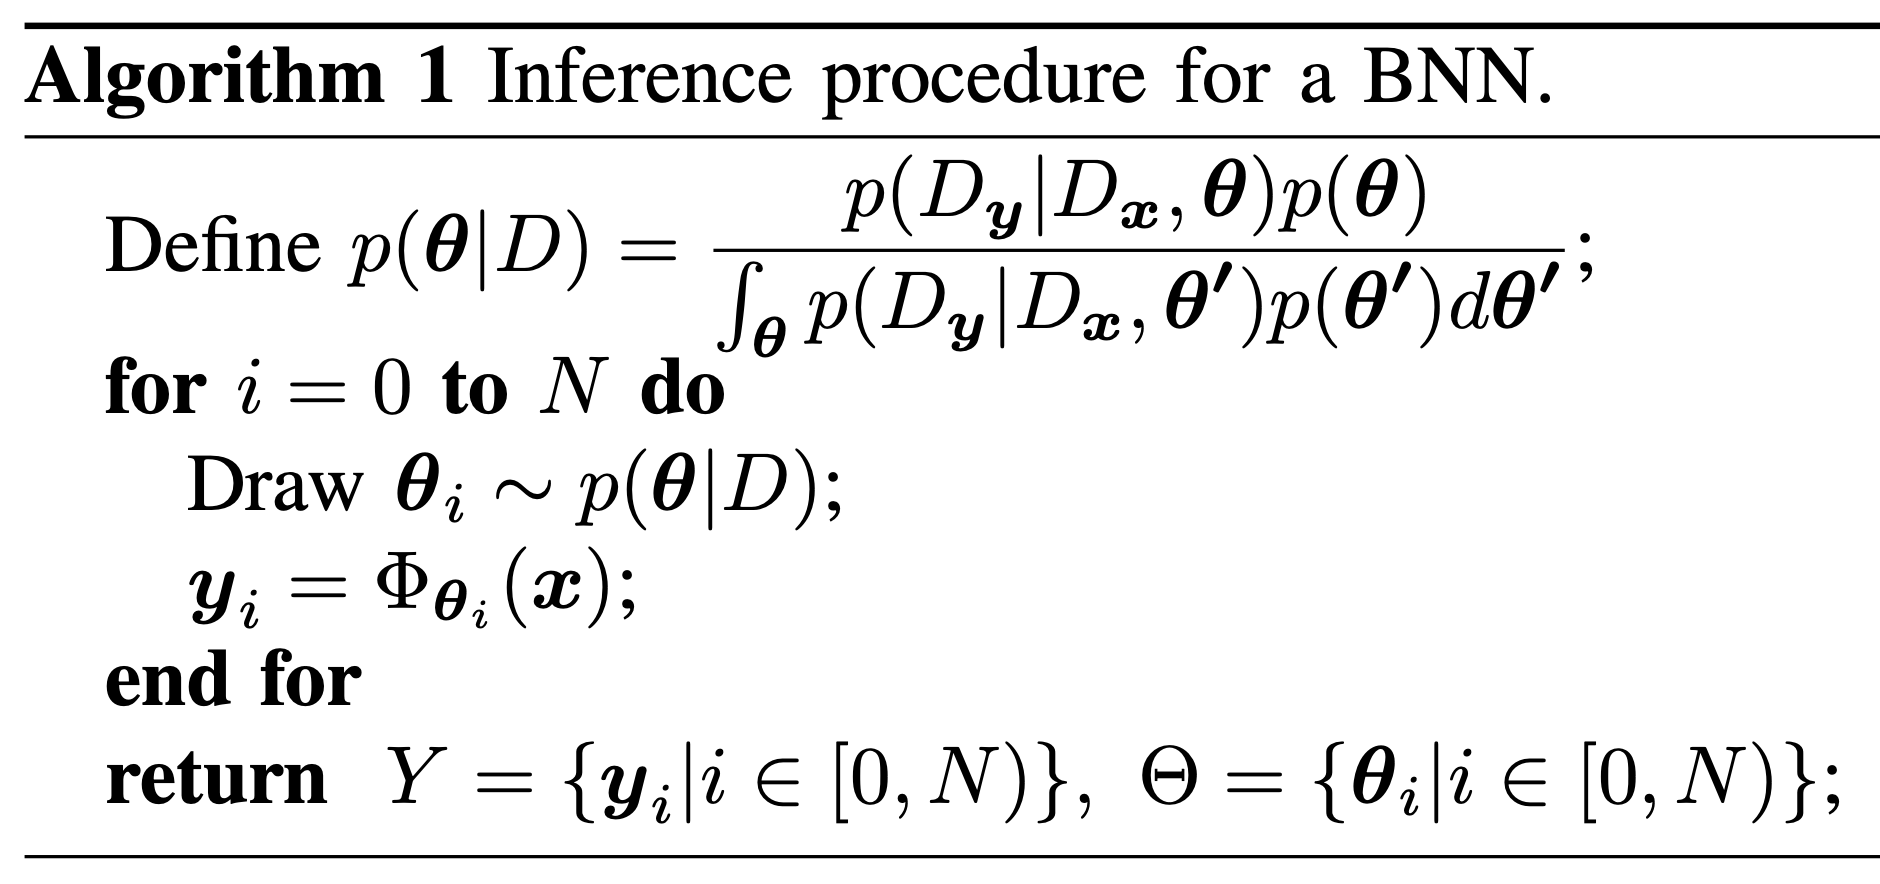
\includegraphics[width=.8\textwidth]{figures_julyan/bdl/hands-on/algo1}
\end{center}
\end{frame}

\begin{frame}{Posterior Sampling Algorithms}
Within the realm of Markov chain Monte Carlo~\citep[MCMC;][]{brooks2011handbook} for BDL, \alert{stochastic gradient MCMC}~\citep[SG-MCMC;][]{nemeth2021stochastic} algorithms, such as stochastic gradient Langevin dynamics~\citep[SG-LD;][]{welling2011bayesian} and stochastic gradient HMC~\citep[SG-HMC;][]{chen2014stochastic}, have emerged as widely adopted tools. 
\begin{itemize}[<+->]
	\item Despite offering \alert{improved posterior approximations}, SG-MCMC algorithms exhibit \alert{slower convergence compared to SGD}~\citep{Robbins1951ASA} (to thoroughly explore the posterior distribution beyond locating the mode). 
	\item A step forward in this regard would be to learn from the machine learning and systems community how to make Monte Carlo faster using \alert{contemporary hardware}~\citep{zhang2022low,wang2023enhancing}. % (YL).
	\item Algorithms such as \alert{Stein variational gradient descent}~\citep[SVGD;][]{liu2016stein} occupy a \alert{middle ground between optimization and sampling}, by employing optimization-type updates but with a set of interacting particles. While recent advances show promising results in BNN settings~\citep{dangelo2021stein, dangelo2021repulsive, pielok2022approximate}, these methods often perform poorly in high-dimensional problems.
	\item Alternatively, posterior exploration can be improved with cyclical step-size schedules~\citep{zhang2019cyclical}.
\end{itemize}
\end{frame}


\begin{frame}{Monte Carlo dropout}
\alert{Dropout} technique reinterpreted as a form of approximate Bayesian variational inference \citep{kingma2015variational,gal2016dropout}.

\alert{Idea}: performing random sampling at test time. Instead of turning off the dropout layers at test time (as is usually done), \alert{hidden units} are randomly dropped out according to a \alert{Bernoulli$(p)$} distribution. Repeating this operation $M$ times provides $M$ versions of the MAP estimate of the network parameters $\bw^m$, $m=1,\ldots,M$ (where some units of the MAP are dropped), yielding an approximate posterior predictive in the form of the equal-weight average:
\begin{equation*}
%\label{eq:MCdropout_post_pred}
	p(y\vert x, \mathcal{D}^n)\approx \frac{1}{M}\sum_{m=1}^M p(y\vert x, \bw^m).
\end{equation*}

\vfill 

\begin{itemize}[<+->]
	\item Monte Carlo dropout captures some uncertainty from out-of-distribution (OOD) inputs
	\item But... \alert{does not provide valid posterior uncertainty}
	\item \citet{folgoc2021mc} show that the Monte Carlo dropout posterior predictive assigns \alert{zero probability} to the true model posterior predictive distribution
\end{itemize}
\end{frame}

\subsection{Tempered and Cold Posteriors}

\begin{frame}{Tempered and Cold Posteriors}
\begin{block}{Tempered posterior}
	A \alert{tempered posterior distribution} with \alert{temperature parameter} $\alert{T}>0$ is defined as $$p(\bw|D) \propto \exp(U (\bw)/\alert{T} )$$ where $U(\bw)$ is the posterior energy function
\begin{equation*}
 U(\bw) :=  \log p(\mathcal{D} | \bw) + \log p(\bw),
\end{equation*}
\end{block}

\pause

\begin{block}{Cold posterior effect}
Empirical evidence \citep{wenzel2020good} that posteriors  exponentiated to some power greater than one (or, equivalently, dividing the energy function $U(\bw)$ by some temperature $T<1$), \alert{performs better} than an untempered one.
\end{block}
\end{frame}
	
\subsection{Prior Specification}

\begin{frame}{Prior Specification}
\begin{itemize}[<+->]
	\item The prior \alert{over parameters} induces a prior \alert{over functions}, and it is the prior over functions that matters for generalization~\citep{wilson2020bayesian}. 
	\item Defining priors over the parameters is hindered by the complexity and unintelligibility of high-dimensional spaces in BDL. 
	\item One aim is to construct informative proper priors on neural network weights that are \alert{computationally efficient} and \alert{favor solutions with desirable model properties}~\citep{vladimirova2019bayesian,fortuin2022bayesian,rudner2023fseb}, such as priors that favor models with 
	\begin{itemize}
		\item reliable uncertainty estimates~\citep{rudner2023uap}, 
		\item a high degree of fairness~\citep{rudner2024gap}, 
		\item generalization under covariate shifts~\citep{klarner2023qsavi}, 
		\item equivariance~\citep{finzi2021residual}, 
		\item or a high level of sparsity~\citep{ghosh2018structured,polson2018posterior,hubin2019combining}.
	\end{itemize}
\end{itemize}
\end{frame}

\subsection{Scalability}

\begin{frame}{Scalability}
\begin{itemize}[<+->]
	\item \alert{Symmetries} in the parameter space of NNs yield \alert{computational redundancies}~\citep{wiese2023}. Addressing the complexity and identifiability issues arising from these symmetries in the context of BDL can significantly impact \alert{scalability}.
	\item Proposed solutions: incorporation of \alert{symmetry-based constraints} in BDL inference methods~\citep{sen2024} or the design of \alert{symmetry-aware priors}~\citep{atzeni2023infusing}. % (TP).
	\item However, removing symmetries may not be an optimal strategy, since part of the success of deep learning can be attributed to the overparameterization of NNs, allowing rapid exploration of numerous hypotheses during training or having other positive `side effects' such as induced sparsity~\citep{kolb2023}. % (DR).
\end{itemize}
\end{frame}


\begin{frame}{Scalability}
\begin{itemize}[<+->]
	\item Although UQ is of significant importance across various domains, it should not come at the cost of \alert{reduced predictive performance}. 
	\item BDL must \alert{strike a balance} by ensuring that the computational cost of UQ matches that of point estimation.
	\item Otherwise, investing computational resources to improve the predictive performance of deep learning models might be a more prudent option. 
	\item Ensembles are less affected by this concern due to their \alert{embarrassingly parallel} nature. 
	\item BUT relying solely on \alert{parallelism} becomes \alert{inadequate} in an era where even industry leaders encounter limitations in graphics processing unit (GPU) resources required to train a single large deep learning model. % (PH).
	\item Simultaneously achieving \alert{time efficiency, memory efficiency, and high model utility} (in terms of predictive performance and uncertainty calibration) remains the \alert{grand challenge} of approximate Bayesian inference. % (YL).
\end{itemize}
\end{frame}


\subsection{Foundation Models}

\begin{frame}{Foundation Models}
\begin{itemize}[<+->]
	\item Deep learning is in the midst of a paradigm shift into the \alert{foundation model} era, characterized by models with \alert{billions, }rather than millions, of parameters, with a predominant focus on \alert{language} rather than vision. 
	\item BDL approaches to LLMs are relatively unexplored, both in terms of methods and applications. 
	\item Only a limited number of works have considered Bayesian approaches to LLMs~\citep{xie2021,cohen2022bayesian, margatina2022,yang2023bayesian}. % (TP), (AGW?).
	\item BDL emerges as a solution to address limitations in foundation models, particularly in scenarios where data availability is limited. In contexts involving \alert{personalized data}~\citep{moor2023foundation} or \alert{causal inference applications}~\citep{zhang2023towards}, such as individual treatment effect estimation, where small datasets prevail, the capacity of BDL for uncertainty estimation aligns seamlessly. 
	\item The \alert{fine-tuning settings} of foundation models in small data scenarios is another example. % (YL).
%
%Thus, foundation models represent a valuable frontier for BDL research, particularly around evaluation and applications. What applications of LLMs or transformers are going to benefit from Bayesian inference tools, such as marginalization and priors? More generally, more meaningful applications are needed to convincingly demonstrate that BDL principles go beyond proof-of-concept.
%The representation of epistemic uncertainty will possibly be most valuable when LLMs or other large-scale NNs are deployed in settings outside of the realm of their training data. For example, Bayesian approaches can be developed and tested in the time series context of applying LLMs in downstream forecasting tasks~\citep{gruver2023}.
\end{itemize}
\end{frame}


\subsection{Diagnostics, Metrics and Benchmarks}

\begin{frame}{Diagnostics, Metrics and Benchmarks}
\begin{itemize}[<+->]
	\item Currently, there is a lack of \alert{convergence} and \alert{performance metrics} specifically for the needs of BDL. Developing such tools can help identify the goals in BDL as well as assess their progress. % (TP).
	\item The choice of \alert{evaluation metrics}, \alert{datasets} and \alert{benchmarks} lack consensus in the BDL community which reflects a difficulty in clearly defining the goals of BDL in a field traditionally viewed through frequentist lens, specifically in terms of performance on test data. % (JA).
	\begin{itemize}[<+->]
	\item \alert{Predictive performance}: ability of the model to give correct answers. Based on metrics, eg: mean square error, risk of 0-1 loss for classification task.
	\item \alert{Model calibration}: assessing that the network is neither overconfident nor underconfident about its prediction. Requires using a test set. Eg: expected calibration error (ECE).
	\end{itemize}
	\item Many of the general Bayesian diagnostic and evaluation approaches are proposed through Bayesian workflow \citep{gelman2020bayesian}, eg with the $\hat R$ diagnostic. 
%\textbf{Convergence diagnostics in parameter space.}
%The analysis of convergence and sampling efficiency~\citep{gelman2013, vehtari2021} for SG-MCMC sampling becomes a delicate matter, which is currently bypassed by a rather simplistic analysis of these quantities using summary statistics of predictive distributions. %(MF).
%More generally, verifying the convergence of inference algorithms in the high-dimensional and multimodal settings of BDL models is not straightforward.
%Convergence checks designed for BNNs need to be further studied.
%
%\textbf{Performance metrics in predictive space.}
%BDL and GP literature often focus on the mean of the predictive distribution, overlooking the analysis of variance of the predictive distribution. Some performance metrics are commonly used to assess variance levels, for example, by evaluating the log-likelihood or the entropy of predictions for test data~\citep{rudner2022fsvi,rudner2023fseb}. However, a systematic way to characterize the predictive uncertainty in BDL inference (apart from binary classification problems where AUROC and AUPRC are widely used) is currently lacking~\citep{arbel2023}. The challenge of setting metrics for the assessment of epistemic and aleatoric uncertainty slows the progress in BDL and could potentially be addressed by establishing widely accepted benchmarks for BDL methods. % (MF).
%
%\textbf{Performance metrics in misspecified settings.}
%Addressing challenges related to distribution shift and test data performance requires the development of robust performance metrics. To establish BDL model reliability under distribution shift, tighter generalization bounds, such as those provided by the PAC-Bayes framework~\citep{langford2002pac, parrado2012pac}, are crucial to obtain probabilistic guarantees on model performance. Furthermore, in misspecified settings, evaluating calibration becomes paramount. Innovative techniques, such as two-stage calibration~\citep{guo2017calibration} and conformal prediction~\citep{papadopoulos2007conformal} or its Bayesian counterpart~\citep{hobbhahn2022fast}, offer practical solutions by refining predicted probabilities and quantifying predictive uncertainty, respectively. These approaches collectively contribute to a more comprehensive evaluation of model performance in scenarios where the underlying assumptions may not align with the true data distribution.
\end{itemize}
\end{frame}


%\begin{frame}{}
%\begin{itemize}[<+->]
%	\item
%\end{itemize}
%\end{frame}
%
%


%%%%%%%%%%%%%%%%%%%%%%%%%%%%%%%%%%%%%%%%%%%%%%%%%%%%%%%%
\section{Priors for Bayesian neural networks}
%%%%%%%%%%%%%%%%%%%%%%%%%%%%%%%%%%%%%%%%%%%%%%%%%%%%%%%%

\subsection{Connection prior-initialization}

\begin{frame}{Connection prior-initialization}
	\alert{At initialization:}
	\begin{itemize}
		\item random weights and biases, e.g., $W^{(l)}_{ij} \sim \mathcal{N}(0, \sigma_w^2)$, 
		$B^{(l)}_{i} \sim \mathcal{N}(0, \sigma_b^2)$;
		\item inputs $X^{(1)}$ fixed.
	\end{itemize} 

	\bigskip
	
	\alert{Goal:}
	\begin{itemize}
		\item find a criterion that the pre-activations $Z^{(l)}$ should match;  \\
			example: $\mathrm{Var}(Z^{(l)}) = 1$;  
		\item deduce a constraint over the distributions of $W^{(l)}$ and $B^{(l)}$;  \\
			example: provided that $W^{(l)}_{ij} \sim \mathcal{N}(0, \sigma_w^2)$, 
			$B^{(l)}_{i} \sim \mathcal{N}(0, \sigma_b^2)$, tune $\sigma_w^2$ and $\sigma_b^2$ accordingly.
	\end{itemize} 
\end{frame}


\begin{frame}{Find a good initialization procedure}
	\alert{Naive heuristic.} (\emph{Understanding the difficulty of training deep feedforward neural 
	networks}, Glorot and Bengio 2010):
	\begin{itemize}
		\item idea: preserve the variance of the pre-activations $Z^{(l)}$;
		\item tune $\sigma_w^2$ and $\sigma_b^2$ s.t.: $\mathrm{Var}(Z^{(l + 1)}) = 
		\mathrm{Var}(Z^{(l)})$. 
	\end{itemize}
	Constraint: the NN is linear ($\phi = \mathrm{Id}$).  \\
	Result: $\sigma_b^2 = 0$, $\sigma_w^2 = 1$, $\mathrm{Var}(\frac{1}{\sqrt{n_l}} W_{ij}^l) = 1$.

	
	\bigskip
	
	\alert{Remark:} this heuristic can be extended to $\phi = $ReLU. \\
	(\emph{Delving deep into rectifiers: Surpassing human-level performance on imagenet classification}, He et al.,  
	2015)  \\
	Result: $\sigma_w^2 = 2$.
\end{frame}

\subsection{Neural-network Gaussian process (NN-GP), Gaussian hypothesis}

\begin{frame}{Neural-network Gaussian process (NN-GP)}
	\begin{itemize}
		\item 	A neural network with one hidden layer, whose width goes to infinity, and which has a Gaussian prior on all the parameters, converges to a Gaussian process with a well-defined kernel \citep{neal1996bayesian}.
	\end{itemize}
	\alert{Proof}: $H$ the number of hidden units, $\phi$ some nonlinear activation function, $b$ biais, weights $v$ and $\boldsymbol{u}$; then unit $k$ can be written
		$$f_k(\boldsymbol{x}) = b_k+\sum_{j=1}^H v_{jk}h_j(\boldsymbol{x}), \quad h_j(\boldsymbol{x}) = \phi(U_{0j}+\boldsymbol{x}^t \boldsymbol{u}_j)$$
		Then
		\begin{itemize}
			\item $\mathbb{E}[f_k(\boldsymbol{x})]=$
			\item $\mathbb{E}[f_k(\boldsymbol{x})f_k(\boldsymbol{x}')]=\ldots := \mathcal{K}(\boldsymbol{x},\boldsymbol{x}')$
			\item The joint distribution over $\{f_k(\boldsymbol{x_n}), n=1:N\}$ converges to a multivariate Gaussian.
			\item So the NN converges to a GP with mean 0 and kernel $\mathcal{K}$, called the \alert{neural network kernel}. It is a non-stationary kernel.
		\end{itemize}
\end{frame}


\subsection{Neural tangent kernel (NTK)}

\begin{frame}{Neural tangent kernel (NTK)}
\begin{itemize}
	\item The NNGP is obtained under the assumption that weights are random and width goes to infinity.
	\item Natural question: can we derive a kernel from a DNN while it is being trained?
	\item The answer is yes \citep{jacot2018neural}. The associated kernel $\mathcal{T}(\boldsymbol{x},\boldsymbol{x}')$ is called the \alert{Neural tangent kernel} (NTK)
	$$\mathcal{T}(\boldsymbol{x},\boldsymbol{x}') := \nabla_{\boldsymbol{\theta}}f(\boldsymbol{x}; \boldsymbol{\theta_\infty})\cdot \nabla_{\boldsymbol{\theta}}f(\boldsymbol{x}'; \boldsymbol{\theta_\infty})$$
	and is obtained with 
	\begin{itemize}
		\item continuous time gradient descent
		\item letting the learning rate $\eta$ become infinitesimally small
		\item letting the widths go to infinity.
	\end{itemize}
\end{itemize}
\end{frame}



\subsection{Edge of Chaos}

\begin{frame}{Edge of Chaos framework}
\alert{See:} \citet{poole2016exponential} and \citet{schoenholz2016deep}

	\medskip
	
	\alert{Main idea.} Let $x_a$ and $x_b$ be two (fixed) inputs:
	\begin{itemize}
		\item variance: $v_a^{(l)} = \mathbb{E} [(Z_{j;a}^{(l)})^2]$;
		\item correlation: $c_{ab}^{(l)} = \frac{1}{\sqrt{v_a^{(l)} v_b^{(l)}}} \mathbb{E}[Z_{j;a}^{(l)} 
		Z_{j;b}^{(l)}]$; 
		\item goal: preserve the correlations $c_{ab}^{(l)}$ during propagation; 
		\item solution: find a recurrence equation $c_{ab}^{(l + 1)} = f(c_{ab}^{(l)})$; 
		\item to do so, we must make an assumption on the distribution of $Z_{j;a}^{(l)}$; \\
			$\Rightarrow$ Gaussian hypothesis: $Z_{j;a}^{(l)} \sim \mathcal{N}(0, v_a^{(l)})$; \\
			Central Limit Theorem ($n_{l} \rightarrow \infty$): $ Z^{(l + 1)}_{j;a} = \frac{1}{\sqrt{n_{l}}}W_j^{(l)} 
			X_a^{(l)} + B^{(l)}_j$; 
		\item resulting simplified dynamics: 
			\begin{align*}
				v_{a}^{(l + 1)}&= \mathcal{V}(v_{a}^{(l)} | \sigma_w, \sigma_b), & c_{ab}^{(l + 1)} &= 
				\mathcal{C}(c_{ab}^{(l)}, v_a^{(l)}, v_b^{(l)} | \sigma_w, \sigma_b) .
			\end{align*}
	\end{itemize}
\end{frame}

\begin{frame}{Edge of Chaos results (Poole et al., 2016; Schoenholz et al., 2016)}
	\alert{Additional assumptions.}
	\begin{itemize}
		\item the sequence $(v_a^{(l)})_l$ tends to a non-zero limit $v^*$, independent from the starting point 
		$v_a^{(0)}$;
		\item $(v_a^{(l)})_l$ is assumed to have already converged; 
		\item so: $c_{ab}^{(l + 1)} = \mathcal{C}(c_{ab}^{(l)}, v^*, v^* | \sigma_w, \sigma_b) = 
		\mathcal{C}_*(c_{ab}^{(l)} | \sigma_w, \sigma_b)$.
	\end{itemize} 
	
	\medskip
	
	\alert{Phases of information propagation:}
	\begin{itemize}
		\item \emph{chaotic phase}: $\lim_{l \rightarrow \infty} c_{ab}^{l} = c^{*} < 1$ \\
			$\Rightarrow$ decorrelate (partially or fully);
		\item \emph{ordered phase}: $\lim_{l \rightarrow \infty} c_{ab}^{l} = c^{*} = 1$ with 
		$\mathcal{C}_*'(1) < 1$ \\
			$\Rightarrow$ correlate fully at an exponential rate;
		\item \emph{edge of chaos}: $\lim_{l \rightarrow \infty} c_{ab}^{l} = c^{*} = 1$ with 
		$\mathcal{C}_*'(1) = 1$ \\
			$\Rightarrow$ correlate fully at sub-exponential rate. 
	\end{itemize}
	$\Rightarrow$ tune $\sigma_w$ and $\sigma_b$ such that the NN lies in the ``edge of chaos'' phase.
\end{frame}


\begin{frame}[allowframebreaks]{Edge of Chaos}
\citet{poole2016exponential} and  \citet{schoenholz2016deep} \begin{figure}[h]
\begin{center}
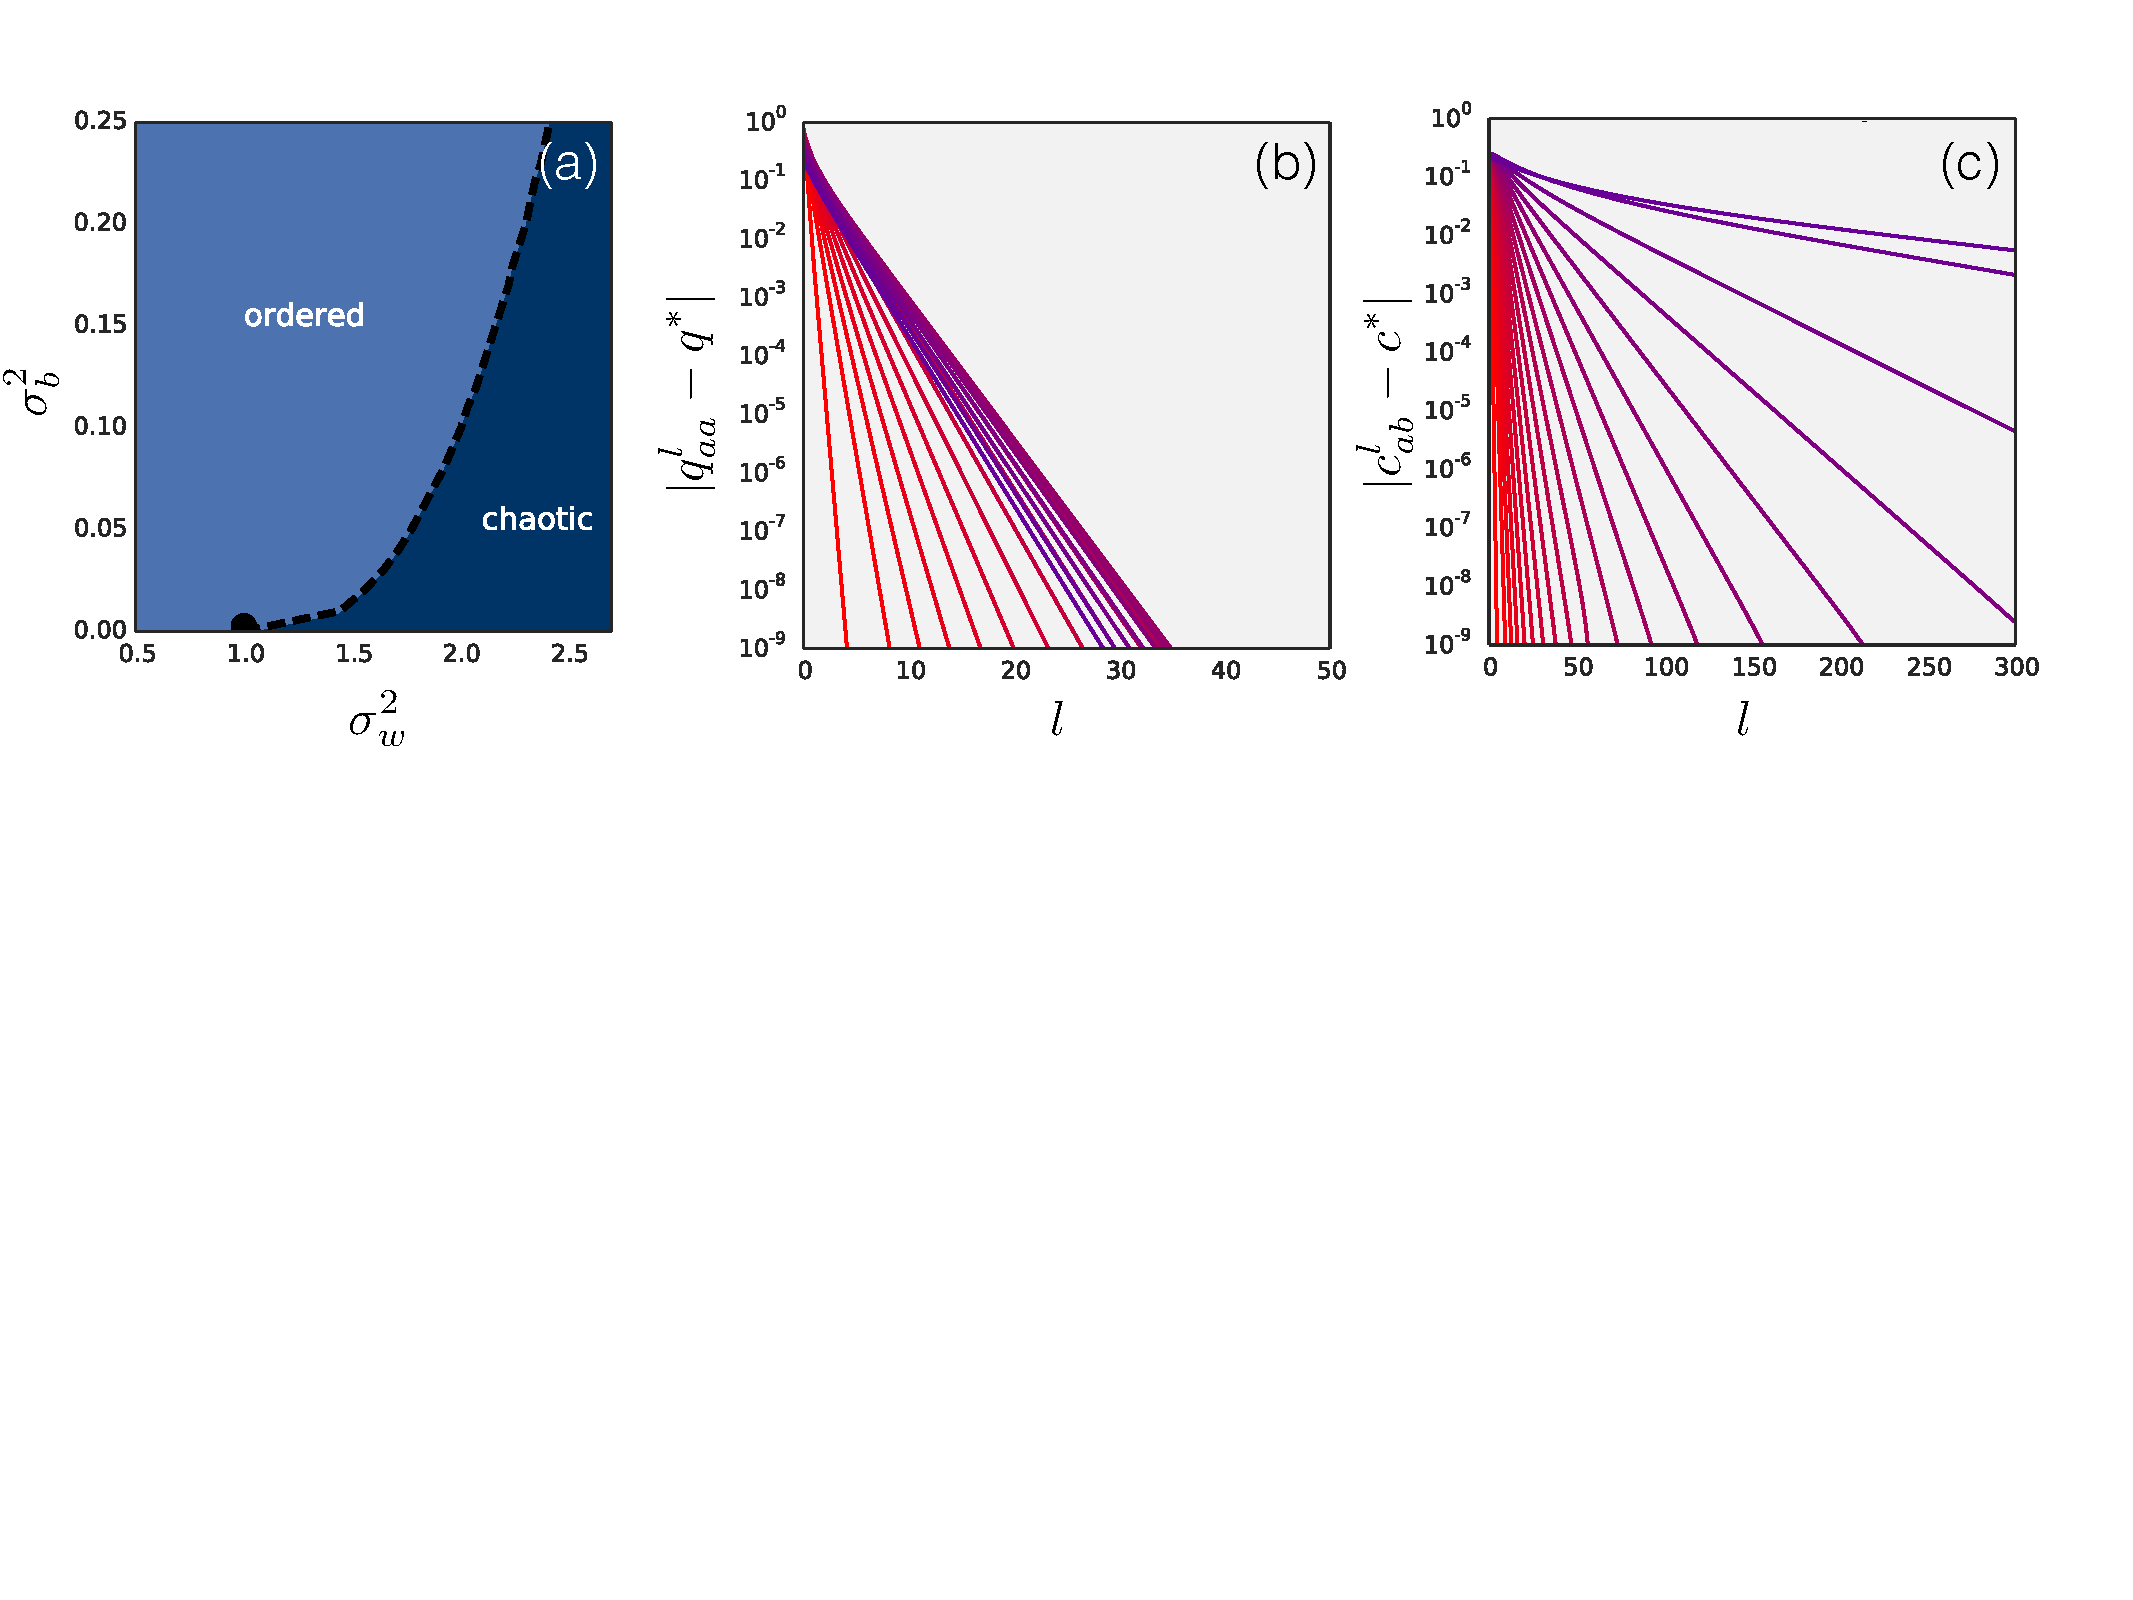
\includegraphics[width=\linewidth]{figures_julyan/bdl/figure_1}
\caption{(a) Edge of chaos diagram showing the boundary between ordered and chaotic phases as a function of $\sigma_w^2$ and $\sigma_b^2$. (b) The residual $|q^* - q_{aa}^l|$ as a function of depth on a log-scale with $\sigma_b^2 = 0.05$ and $\sigma_w^2$ from 0.01 (red) to 1.7 (purple). Clear exponential behavior is observed. (c) The residual $|c^* - c_{ab}^l|$ as a function of depth on a log-scale. Again, the exponential behavior is clear. The same color scheme is used here as in (b).  \label{fig:phase_diagram}}
\end{center}
\hfill\textcolor{gray}{From \citet{schoenholz2016deep}}
\end{figure}


\end{frame}


\subsection{Unit priors get heavier with depth}

\begin{frame}{Understanding priors at the unit level}
	\begin{definition}[Generalized Weibull-tail on $\mathbb{R}$]
\label{def:gen_weibull-tail_r}
A random variable $X$ is generalized Weibull-tail on $\mathbb{R}$ with tail parameter $\beta > 0$ if both its right and left tails are upper and lower bounded by some Weibull-tail functions with tail parameter~$\beta$:
\begin{align*}
    \edr^{-x^{\beta} l_1^r(x)} \le & \overline{F}_X(x) \le \edr^{-x^{\beta} l_2^r(x)}, \quad \ \ \ \text{for }x > 0 \text{ and $x$ large enough}, \\
    \edr^{-|x|^{\beta} l_1^l(|x|)} \le & F_X(x) \le \edr^{-|x|^{\beta} l_2^l(|x|)}, \quad \text{for } x < 0 \text{ and $-x$ large enough},
\end{align*}
where $l_1^r$, $l_2^r$, $l_1^l$ and $l_2^l$ are slowly-varying functions. 
We note $X \sim GWT(\beta)$. 
\end{definition}
\end{frame}

\begin{frame}{Understanding priors at the unit level}
This tail description reveals the difference between hidden units' distributional properties in finite- and infinite-width Bayesian neural networks, since 
hidden units are generalized Weibull-tail with a tail parameter depending on those of the weights:
\begin{theorem}[\citealp{vladimirova2021accurate}]
\label{theorem:hidden_units_are_gwt}
Consider a Bayesian neural network  with ReLU activation function. Let $\ell$-th layer weights be independent symmetric generalized Weibull-tail on~$\mathbb{R}$ with tail parameter $\beta^{(\ell)}_w$. 
Then conditional on the input $\bx$, the marginal prior distribution induced by forward propagation on any pre-activation is generalized Weibull-tail on~$\mathbb{R}$: for any $1\leq \ell\leq L$, and for any $1\leq m\leq H_\ell$,
$$g_m^{(\ell)}\sim GWT(\beta^{(\ell)}),$$
with tail parameter $\beta^{(\ell)}$ such that $\frac{1}{\beta^{(\ell)}} = \frac{1}{\beta^{(1)}_w} + \dots + \frac{1}{\beta^{(\ell)}_w}$.
\end{theorem}
Note that the most popular case of weight prior, iid Gaussian \citep{neal1996bayesian}, corresponds to $\text{GWT}_{\mathbb{R}}(2)$ weights. This leads to units of layer $\ell$ which are $\text{GWT}_{\mathbb{R}}(\frac{2}{\ell})$. 
\end{frame}

\begin{frame}{Understanding priors at the unit level}


\def\bW{\boldsymbol{W}}
\def\bU{\boldsymbol{U}}
\def\Lnorm{\mathcal{L}}

\begin{center}
\begin{tabular}{@{}cclc@{}}
\toprule
Layer                         & Penalty on $\bW$         & \multicolumn{2}{c}{Approximate penalty on $\bU$}         \\ \toprule
$1$ & $\Vert \bW^{(1)}\Vert_2^{2}$, $\Lnorm^2$   & $\Vert \bU^{(1)}\Vert_2^{2}$ & $\Lnorm^2$  (weight decay)\\%\hline
$2$ & $\Vert \bW^{(2)}\Vert_2^{2}$, $\Lnorm^2$   & $\Vert \bU^{(2)}\Vert$ & $\Lnorm^1$  (Lasso)\\%\hline
% \vdots &\vdots &\vdots \\
$\ell$ & $\Vert \bW^{(\ell)}\Vert_2^{2}$, $\Lnorm^2$   & $\Vert \bU^{(\ell)}\Vert_{2/\ell}^{2/\ell}$ & $\Lnorm^{2/\ell}$ \\ 
% $\ell = L$ & $\Vert \bW^{(L)}\Vert_2^{2}$, $\Lnorm^2$   & $\Vert \bU^{(L)}\Vert_{2/L}^{2/L}$, $\Lnorm^{2/L}$ \\ 
\bottomrule
\end{tabular}\bigskip 

  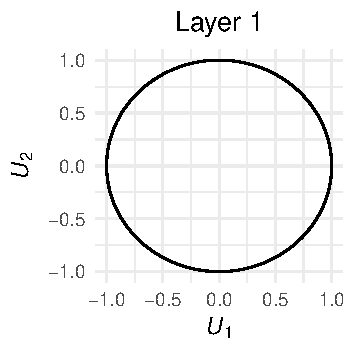
\includegraphics[width=.32\textwidth]{figures_julyan/bdl/001}
  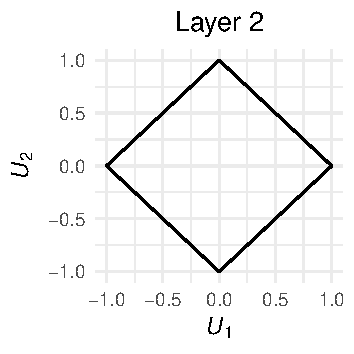
\includegraphics[width=.32\textwidth]{figures_julyan/bdl/002}
  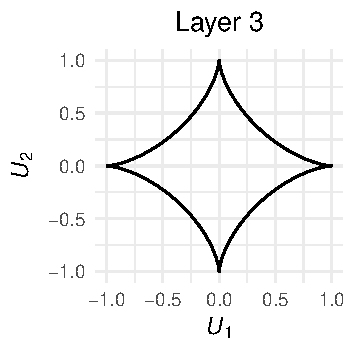
\includegraphics[width=.32\textwidth]{figures_julyan/bdl/003}

\end{center}

\end{frame}

%\subsection{Other priors}
%
%
%
%\begin{frame}{Other priors}
%\begin{itemize}
%	\item Although Gaussian priors are simple and widely used, they are not the only option. 
%	\item For some applications, it is useful to use shrinkage or sparsity promoting priors which encourage most of the weights to be small/close to zero. Examples of such priors
%	\begin{itemize}
%	 \item  Laplace prior
%	$$p_\lambda(x) = \frac{\lambda}{2}e^{-\lambda|x|}.$$
%		\item spike-and-slab
%	\end{itemize}
%\end{itemize}
%
%\end{frame}






%%%%%%%%%%%%%%%%%%%%%%%%%%%%%%%%%%%%%%%%%%%%%%%%%%%%%%%%%
%\section{Inference algorithms}
%%%%%%%%%%%%%%%%%%%%%%%%%%%%%%%%%%%%%%%%%%%%%%%%%%%%%%%%%
%\begin{frame}
%	
%\end{frame}
%
%\begin{frame}{Bayesian inference: basic sampling algorithm}
%Denote data by $D=\{D_x,D_y\}$ and parameters (weights) by $\boldsymbol{\theta}$.
%\begin{center}
%	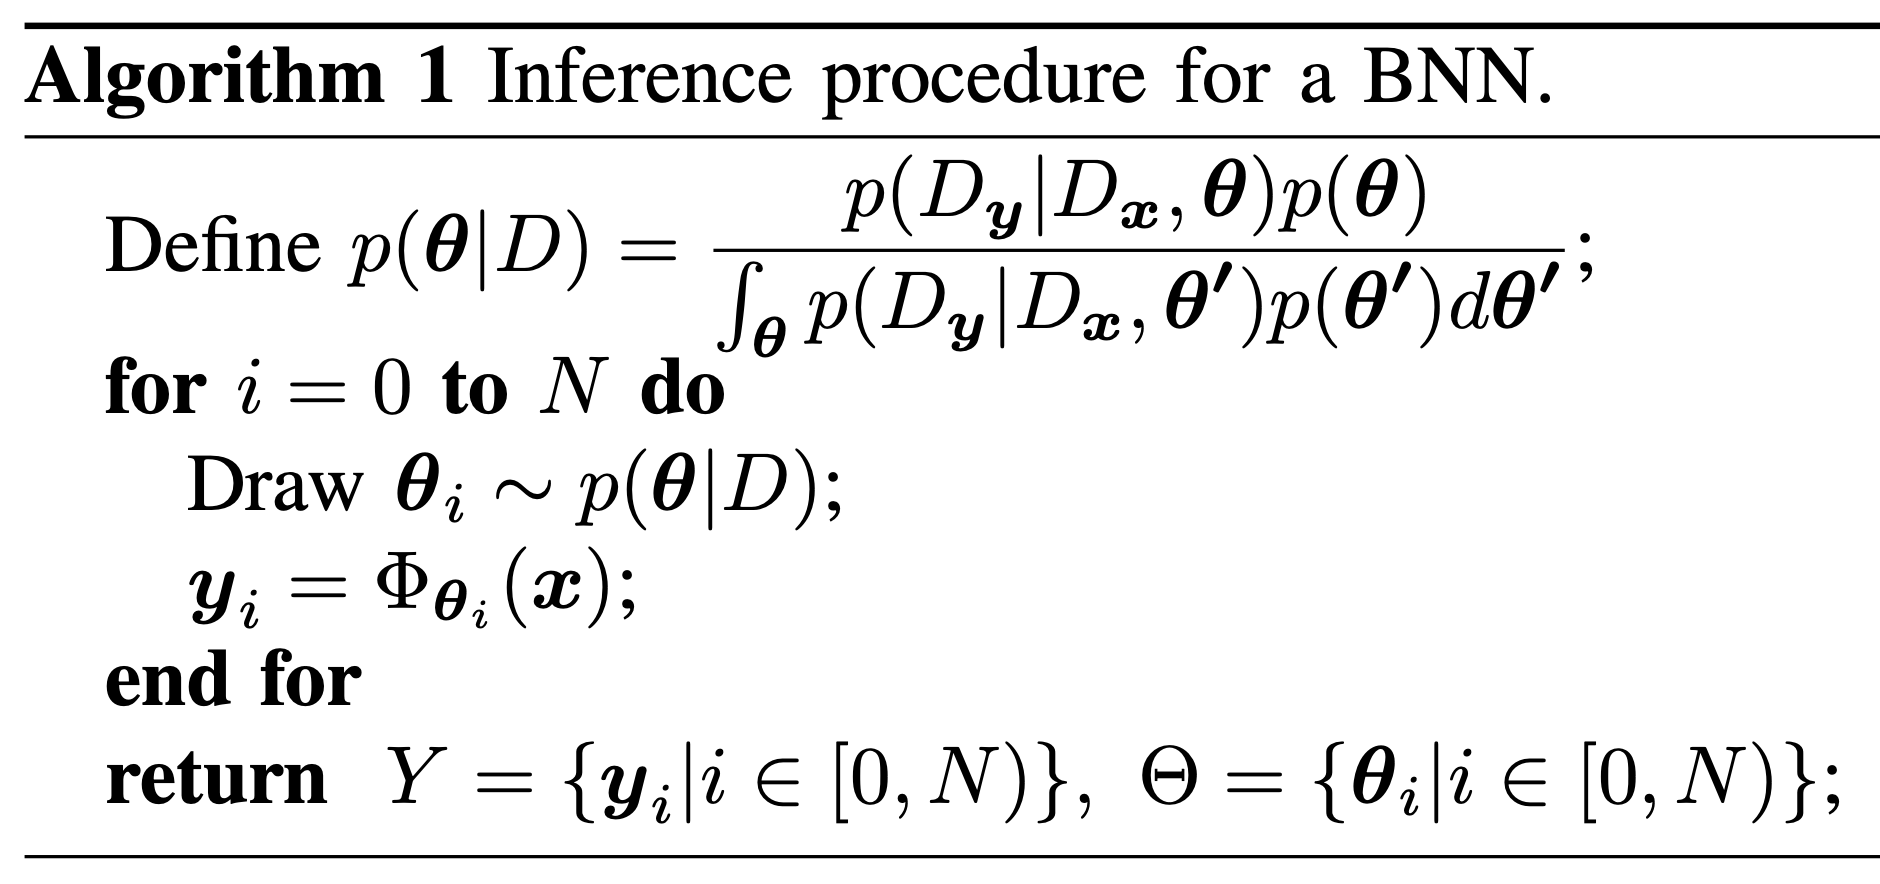
\includegraphics[width=.8\textwidth]{figures_julyan/bdl/hands-on/algo1}
%\end{center}
%\end{frame}
%
%
%
%\begin{frame}{Laplace approximation}
%Computes a Gaussian approximation to the posterior centered at the MAP estimate
%
%\begin{itemize}
%	\item It is simple
%	\item But... computing the Hessian is expensive, and may result in a non-positive definite matrix since the log likelihood of deep neural networks is non-convex.
%	\item Gauss--Newton approximation to the Hessian
%\end{itemize}
%
%\begin{block}{Generalized Gauss--Newton approximation}
%	$$\bH^{\mathrm{GGN}}:= \sum_{i=1}^n \mathcal{J}_{\bw}(\bx_i)^{\top}\boldsymbol{\Lambda}(\by_i;f_i)\mathcal{J}_{\bw}(\bx_i),$$
%where $\mathcal{J}_{\bw}(\bx)$ is the network per-sample Jacobian $\left[\mathcal{J}_{\bw}(\bx)\right]_{c}=\nabla_{\bw}f_c(\bx;\bw_{\hat{\rho}})$, and $\boldsymbol{\Lambda}(\by;f)=-\nabla^2_{ff}\log p(\by;f)$ is the per-input noise matrix.% \citep{kunstner2019limitations}.
%\end{block}
%
%\end{frame}
%
%
%
%
%\begin{frame}{Bayesian neural networks: early algorithms}
%\begin{itemize}[<+->]
%	\item \alert{Markov chain Monte Carlo} (MCMC), \alert{Hamiltonian Monte Carlo} (HMC). No-U-Turn sampler (NUTS) it most often used in probabilistic programming languages (Stan, PyMC3, Pyro, etc): is improves over classic HMC by allowing hyperparameters to be set automatically instead of manually
%	\item \alert{Variational inference} (VI): scales better than MCMC algorithms. Idea: find an approximate variational distribution in a variational family that is as close as possible to the exact posterior by minimizing the Kullback--Leibler divergence. Turns sampling into optimization.
%	\item \alert{Stochastic variational inference} (SVI): scales better than VI, stochastic gradient descent method applied to VI. Gradient of objective is computed only on mini-batches.
%\end{itemize}
%\end{frame}
%
%
%
%
%\begin{frame}{Bayesian neural networks: early algorithms}
%\begin{alertblock}{BUT}
%	Stochasticity in gradient estimation stops backpropagation from functioning
%\end{alertblock}
%\pause
%
%
%\begin{block}{Tricks for Monte Carlo gradient estimation}
%	A number of \alert{tricks} \citep[see][]{mohamed2020montecarlo}
%	\begin{itemize}[<+->]
%		\item Log-derivative trick: score function estimators
%		\item Reparameterisation trick: pathwise derivative estimator
%		\item Measure-valued gradient estimators
%	\end{itemize}
%\end{block}
%\end{frame}
%
%
%
%\begin{frame}{Bayesian neural networks: adapted algorithms}
%\begin{itemize}[<+->]
%	\item \alert{Bayes-by-backprop} (BBB) and \alert{probabilistic backpropagation} (PBP): implement the reparameterisation trick
%	\item \alert{Monte Carlo dropout}: turning dropout into an approximate Bayesian algorithm (variational inference)
%	\item  \alert{Bayes via stochastic gradient descent}: includes MCMC algorithms based on the SGD dynamic such as stochastic gradient Langevin dynamic (SGLD) and Variational Inference based on SGD dynamic such as ensembling
%\end{itemize}
%\end{frame}
%
%
%\begin{frame}[allowframebreaks]{Monte Carlo dropout}
%Dropout technique reinterpreted as a form of approximate Bayesian variational inference \citep{kingma2015variational,gal2016dropout}.
%
%\alert{Idea}: performing random sampling at test time. Instead of turning off the dropout layers at test time (as is usually done), \alert{hidden units} are randomly dropped out according to a \alert{Bernoulli$(p)$} distribution. Repeating this operation $M$ times provides $M$ versions of the MAP estimate of the network parameters $\bw^m$, $m=1,\ldots,M$ (where some units of the MAP are dropped), yielding an approximate posterior predictive in the form of the equal-weight average:
%\begin{equation*}
%%\label{eq:MCdropout_post_pred}
%	p(y\vert x, \mathcal{D}^n)\approx \frac{1}{M}\sum_{m=1}^M p(y\vert x, \bw^m).
%\end{equation*}
%
%\vfill 
%
%\begin{itemize}[<+->]
%	\item Monte Carlo dropout captures some uncertainty from out-of-distribution (OOD) inputs
%	\item But... \alert{does not provide valid posterior uncertainty}
%	\item \citet{folgoc2021mc} show that the Monte Carlo dropout posterior predictive assigns \alert{zero probability} to the true model posterior predictive distribution
%\end{itemize}
%\end{frame}
%
%
%\begin{frame}{Tempered and cold posteriors}
%\begin{block}{Tempered posterior}
%	A \alert{tempered posterior distribution} with \alert{temperature parameter} $\alert{T}>0$ is defined as $$p(\bw|D) \propto \exp(U (\bw)/\alert{T} )$$ where $U(\bw)$ is the posterior energy function
%\begin{equation*}
% U(\bw) :=  \log p(\mathcal{D} | \bw) + \log p(\bw),
%\end{equation*}
%\end{block}
%
%\pause
%
%\begin{block}{Cold posterior effect}
%Empirical evidence \citep{wenzel2020good} that posteriors  exponentiated to some power greater than one (or, equivalently, dividing the energy function $U(\bw)$ by some temperature $T<1$), \alert{performs better} than an untempered one.
%\end{block}
%
%
%
%\end{frame}


\section{Proposed Future Directions}

%Ongoing research initiatives dedicated to addressing the challenges of BDL, particularly focusing on scalability. 

\subsection{Posterior Sampling Algorithms}

\begin{frame}
\frametitle{Advancements in Posterior Sampling Algorithms}

\begin{itemize}
    \item Emerging need for new classes of posterior sampling algorithms for improved performance on DNNs.
    \item Objectives: Enhance efficiency, reduce computational overhead, and enable effective high-dimensional exploration.
\end{itemize}

\textbf{Innovative Approaches:}
\begin{itemize}
    \item SG-MCMC with tempered posteriors for multi-mode sampling challenges.
    \item Development based on optimal transport theory~\citep{villani2021topics}, score-based diffusion models~\citep{song2020score}, and ODE approaches like flow matching~\citep{lipman2022flow}.
    \item Utilization of NNs for mapping complex data distributions or in MCMC proposal mechanisms.
\end{itemize}

\end{frame}

\begin{frame}
\frametitle{Strategies for Enhancing Posterior Sampling}

\textbf{Cross-Mode Exploration and Identifiability:}
\begin{itemize}
    \item SG-MCMC algorithms to traverse isolated modes rapidly, possibly via normalizing flows.
    \item Incorporating constraints for identifiability and focusing on identifiable functionals~\citep{gu2023}.
\end{itemize}

\textbf{Subspace Approaches and Future Directions:}
\begin{itemize}
    \item SG-MCMC in parameter space subspaces (linear, sparse)~\citep{izmailov2020,li2023training}.
    \item Formulating uncertainty statements for targeted subnetworks and beyond~\citep{dold2024}.
    \item Hybrid samplers combining structured variational inference with MCMC for efficiency~\citep{alexos2022structured}.
    \item Exploring subsampling and transfer learning integration~\citep{kirichenko2023last}.
\end{itemize}

\end{frame}

%
%There is a need for new classes of posterior sampling algorithms that perform better on deep neural networks (DNNs). These algorithms should aim to enhance efficiency, reduce computational overhead, and enable more effective exploration of high-dimensional parameter spaces.
%
%SG-MCMC with tempered posteriors may potentially overcome the issue of sampling from multiple modes. This could be achieved by developing new sampling approaches that can be based on ideas from optimal transport theory~\citep{villani2021topics}, score-based diffusion models~\citep{song2020score}, and ordinary differential equation (ODE) approaches such as flow matching~\citep{lipman2022flow}, which use NNs to learn a mapping from a simpler (usually Gaussian) distribution to a complex data distribution (for example, a distribution of images). So, one could plausibly use an NN either to learn a mapping between the BDL posterior and a Gaussian distribution or to use an NN in an MCMC proposal mechanism. % (CN).
%
%Generally, instead of just focusing on local information about the posterior, there is a need for SG-MCMC algorithms that are able to move rapidly across isolated modes, for instance, using normalizing flows. Since one may not expect to accurately approximate a high-dimensional posterior with respect to all the BNN parameters, novel performance metrics may target lower-dimensional functionals of interest, including UQ as a key piece.
%
%One approach is to incorporate appropriate constraints to attain identifiability, for instance, by doing inference on the latent BNN structure~\citep{gu2023}. Instead, one can focus on identifiable functionals for canonical classes of NNs, targeting posterior approximation algorithms for these functionals. Further, one may consider decoupling approaches, which use the BNN as a black box to fit the data-generating model and then choose appropriate loss functions to conduct inference in a second stage. % (DD).
%
%Another promising approach is running SG-MCMC algorithms in subspaces of the parameter space, for example, linear or sparse subspaces~\citep{izmailov2020,li2023training}, further enabling the formulation of uncertainty statements for targeted subnetworks~\citep{dold2024}. In the future, SG-MCMC operating on QLoRA~\citep{dettmers2023} or non-linear subspaces may be constructed. Besides treating subspaces deterministically, posterior dependencies between subspaces can be broken systematically, leading to novel hybrid samplers that combine structured variational inference with MCMC~\citep{alexos2022structured} to achieve compute-accuracy trade-offs.
%Subsampling for BDL can be combined with reasoning about transfer learning~\citep{kirichenko2023last}. % (AGW).

\subsection{Hybrid Bayesian Approaches}

\begin{frame}
\frametitle{Hybrid Bayesian Approaches: An Overview}

Future BDL approaches may focus on uncertainty in specific model areas, while others are efficiently estimated using point estimation. Hybrid approaches combine Bayesian methods with the efficiency of deterministic deep learning.

\begin{itemize}
    \item Developing methods that apply Bayesian approaches in critical areas for cost-effective uncertainty capture.
    \item Maintaining deterministic approaches for other model parts~\citep{daxberger2021a}.
    \item Example: Last-layer Laplace approximation~\citep{daxberger2021b}.
\end{itemize}

Such hybrid approaches represent a promising research area.

\end{frame}

\begin{frame}
\frametitle{Advancements and Literature in Hybrid Models}

Traditional combinations of deep learning and GPs have been limited by GP scalability.

\begin{itemize}
    \item Recent advances in GP inference scale-up are promising for broader application of hybrid models~\citep{wilson2016deep}.
    \item Deep Kernel Learning (DKL) as a key example of scalable hybrid models.
\end{itemize}

Prolific literature connects BDL with deep Gaussian processes (DGPs), involving neural network GPs arising as infinite-width limits of NNs.

\begin{itemize}
    \item Connections between NNs and GPs provide valuable insights into BDL theory~\citep{damianou2013,agrawal2020,neal1996,matthews2018}.
\end{itemize}
\end{frame}

%In the future, practical BDL approaches may capture uncertainty over a limited part of the model, while other parts may be estimated efficiently using point estimation. So, one may consider hybrid approaches that combine Bayesian methods with the efficiency of deterministic deep learning.
%
%This could involve developing methods that selectively apply Bayesian approaches in critical areas of the model where capturing uncertainty will be more useful and cheaper, while maintaining a deterministic approach for other parts of the model~\citep{daxberger2021a}. The last-layer Laplace approximation is an example of this~\citep{daxberger2021b}. Such hybrid approaches are a promising area for future research.% (JMHL).
%
%Combinations of deep learning methods and GPs have traditionally been limited by the lack of scalability of GPs. However, recent advances in scaling up GP inference are promising for making these hybrid models more widespread. % (JMHL).
%DKL~\citep{wilson2016deep} is one example of such a hybrid model. The DKL scalability frontier may be further pushed by exploiting advances in GP scalability.% (TP).
%
%There exists a prolific literature on connecting BDL and deep Gaussian processes~\citep[DGPs;][]{damianou2013,agrawal2020}. This line of work involves neural network GPs~\citep{neal1996,matthews2018}, which are GPs that arise as infinite-width limits of NNs. Insights into the theory of BDL may come from the analysis of this connection between NNs and GPs. % (MF).

\subsection{Deep Kernel Processes and Machines}

%Deep kernel processes (DKPs) constitute a promising family of deep non-parametric approaches to BDL~\citep{aitchison2021deep,ober2021variational,ober2023improved}. A DKP is a deep GP, in which one treats the kernels, rather than the features, as random variables. Remarkably, it is possible to write down the prior and perform inference entirely for kernels, without ever needing DGP features or BNN weights~\citep{aitchison2021deep}. Thus, DKPs resolve a pernicious problem with BDL: the highly multimodal posteriors caused by permutation symmetries. It is very difficult to accurately approximate these multimodal posteriors with simplified parametric families, for instance, as used in Laplace or variational inference. In contrast, the DKP posterior in practice seems to be unimodal~\citep{yang2023theory}.
%
%Deep kernel machines~\citep[DKMs;][]{milsom2023convolutional,yang2023theory} go further, by taking the infinite-width limit of a DKP. Usually such an infinite-width limit would eliminate representation learning. However, DKMs carefully temper the likelihood in order to retain representation learning, and are thereby able to attain state-of-the-art predictive performance~\citep{milsom2023convolutional}, while their theoretical implications are profound for BDL. DKMs offer key insights into what we really mean by `inference in function space' and how it relates to representation learning. Specifically, the kernels learned at every layer in a DKM define a `function space' at every layer. In fact, in a DKM, the true posterior over features is multivariate Gaussian with covariance given by the learned kernel~\citep{aitchison2021deep}. Representation learning occurs as these function spaces at every layer are modulated by training to focus on the features that matter for predictive performance.

\subsection{Semi-Supervised and Self-Supervised Learning}

%From a Bayesian perspective, one of the surprises in modern deep learning has been the success of semi-supervised learning, where the objective is seemingly arbitrary (or at least, it does not obviously correspond to a likelihood in a known model). Additionally, in Bayesian inference, there are phenomena such as the `cold posterior effect'~\citep{aitchison2020statistical,wenzel2020}, in which BDL appears to attain more competitive predictive performance by taking the posterior to a power greater than one, thereby shrinking the posterior. In particular, the patterns exploited by semi-supervised learning arise from data curation~\citep{ganev2023}. If semi-supervised learning is performed on uncurated data, any improvements disappear. This casts doubt on the applicability of semi-supervised learning on real-world uncurated datasets. The cold posterior results can also be explained by underconfident aleatoric uncertainty representation~\citep{kapoor2022uncertainty}.  %(LA, AGW).
%
%Self-supervised learning is an alternative to semi-supervised learning. Self-supervised learning is based on objectives such as mutual information between latent representations of two augmentations of the same underlying image. From a Bayesian perspective, these objectives appear to be ad hoc, as they do not correspond to any likelihood. However, it is possible to formulate a rigorous likelihood in the form of a recognition-parameterized model~\citep{aitchison2023}. This provides insight into the workings of self-supervised learning and how to generalize it to new settings, such as viewing it as a way to learn Bayesian priors~\citep{shwartz2022,sharma2023incorporating}. % (LA).

\subsection{Mixed Precision and Tensor Computations}

%The success of deep learning is closely tied to its coupling with modern computing and specialized hardware, leveraging technologies like GPUs. Recent investigations within deep learning on the impact of mixed precision point to a role for Bayes, particularly probabilistic numerics~\citep{oates2019modern}, in making more efficient use of computation. Mixed precision introduces uncertainty into the internal computations of a model, which Bayes can effectively propagate to downstream predictions. Furthermore, mixed precision requires making decisions about which precision to use, where Bayes can ensure that these decisions are optimal and sensitive to the relations between numerical tasks. % (MAO).
%Drawing inspiration from specialized hardware, such as tensor processing units, there is potential for a similar trajectory in BDL to address scalability concerns~\citep{mansinghka2009natively}. This suggests that the creation of dedicated hardware for BDL has the potential to spark a reevaluation of inference strategies. %(MF).
%
%In a parallel vein, accelerating software development is crucial to encouraging deep learning practitioners to adopt Bayesian methods. There is a demand for user-friendly software that facilitates the integration of BDL into various projects. The goal is to make BDL usage competitive in terms of human effort compared to standard deep learning practices. For details on BDL software efforts, see~\cref{sec:software}.

\subsection{Compression Strategies}

%To decrease the computational cost of BDL models, for both memory efficiency and computational speed, compression strategies are being explored. An approach involves using sparsity-inducing priors to prune large parts of BNNs~\citep{louizos2017bayesian}. Alternatively, the prior can serve as an entropy model, enabling the compression of BNN weights~\citep{yang2023introduction}. Methods such as relative entropy coding and variational Bayesian quantization, where the quantization grid is dynamically refined, provide efficient BNN compression~\citep{yang2020}. These novel tools could also be used to dynamically decode a Bayesian ensemble at test time to various levels of precision or ensemble size, resulting in precision-compute trade-offs. 
%
%Furthermore, in the context of compressing NN weights, a viable approach involves obtaining the posterior distribution based on observed data and encoding a sample into a bit sequence to send to a receiver~\citep{havasi2018}.  The receiver can then extract the posterior sample and use the corresponding weights to make predictions. In practice, approximations are needed to obtain the posterior, encode the sample, and use the corresponding weights to make predictions. Despite the need for approximations in the process, this method yields commendable trade-offs between compression cost and predictive quality compared to alternatives centered on deterministic weight compression.
%%(SM)% (JMHL).

%\subsection{Other Future Directions}
%
%
%\textbf{Bayesian transfer and continual learning.}
%The transfer learning paradigm is quickly becoming a standard way to deploy deep learning models. As noted in~\cref{sec:existing-BDL}, BDL is optimized for transfer learning. The focus is not solely on transferring an initialization as in traditional deep learning; instead, knowledge of the source task may inform the shapes and locations of optima on downstream tasks~\citep{rudner2022sfsvi,rudner2023fseb}. Self-supervised learning can also be used to create informative self-supervised priors for transfer learning~\citep{shwartz2022, sharma2023incorporating}. % (AGW).
%Leveraging its efficiency in learning under temporally-changing data distributions through posterior updates, current efforts in the continual learning context explore approaches that integrate new information either assuming a continuous rate of change~\citep{nguyen2018variational, chang2022diagonal} or incorporating priors for changepoint detection~\citep{li2021detecting}.
%
%\textbf{Probabilistic numerics.}
%Probabilistic numerics~\citep{hennig2022probabilistic} is the study of numerical algorithms as Bayesian decision-makers. As numerical algorithms, such as optimization and linear algebra, are clearly central to deep learning, probabilistic numerics offers interesting prospects for making deep learning both more powerful and Bayesian. As one example, since deep training is now regularly I/O-bound for large models, active management of data loading, during training and UQ, is of increasing interest. Methods that quantify and control the information provided by individual computations, based on their effect on the BDL posterior, are showing promise as a formalism for algorithmic data processing in deep training~\citep{tatzel2023accelerating}, using probabilistic numerical linear algebra~\citep{NEURIPS2022_4683beb6} to select sparse informative `views' on the data.
%
%\textbf{Singular learning theory.}
%Singular learning theory~\citep[SLT;][]{wat09} investigates the relation between Bayesian losses, such as approximations of the marginal log-likelihood, and neural network loss functions, using principles from non-equilibrium statistical mechanics. Recent research has drawn connections between Bayesian methods and SLT~\citep{wei23}. %(MW).
%
%\textbf{Conformal prediction.}
%For UQ, alternatives such as conformal prediction have emerged as competitors to Bayesian methods and result in well-calibrated uncertainties~\citep{vovk05}. % (SM).
%Deep learning models can be used to develop conformal prediction algorithms~\citep{meister2023} and, conversely,
%conformal prediction methods can be used to quantify or calibrate uncertainty in deep learning models. % (TP).
%A Bayesian approach to conformal prediction has started to emerge~\citep{hobbhahn2022fast,murphy2023probabilistic}, promising a synergistic approach that combines the strengths of Bayesian reasoning with the well-calibrated UQ offered by conformal prediction.
%
%\textbf{LLMs as distributions.}
%LLMs may be used flexibly as distribution objects in arbitrarily complex programs and workflows. By taking a Bayesian stance, several questions emerge for exploration. When multiple LLMs interact, how does one perform joint inference? What is an effective approach to marginalize over latent variables generated by LLMs, facilitating joint learning over such latent spaces?
%Is it possible to adopt tools from computational statistics or approximate inference to perform various forms of reasoning with LLMs? And are there innovative ways to synergize small and large LLMs to amortize inferences just in time? % (TK)?
%
%\textbf{Meta-models.}
%An intriguing prospect arises when contemplating whether BDL will parallel the trajectory of language models. Could one envision the development of a Bayesian meta-model within the BDL framework~\citep{krueger2017bayesian}? This meta-model, akin to language models, may be fine-tuned to multiple tasks, demonstrating competitive predictive performance across them, thus generalizing approaches in amortized inference~\citep{garnelo2018conditional, gordon2019convolutional,muller2021transformers}. %(MF)?
%
%\textbf{Sequential decision benchmarks.}
%Standard image-based benchmarks focus exclusively on state-of-the-art predictive performance, where non-Bayesian deep learning algorithms typically have an advantage over BDL. To quantify predictive uncertainty, it is encouraged to shift attention to more thorough simulation studies or scientific applications focused on sequential learning and decision-making, such as experimental design, Bayesian optimization, active learning, or bandits. By prioritizing sequential problems in such contexts, researchers and practitioners can gain insights into how well a model generalizes to new and unseen data, how robust it is under uncertain conditions, and how effectively its uncertainty estimates can be utilized by decision makers in real-world scenarios.

\section{Softwares}
%\label{sec:software}

%Applying a BDL approach to a real-world problem is still a more complex endeavor than opting for an off-the-shelf standard deep learning solution, which limits the real-world adoption of BDL. % (VF).
%Software development is key to encouraging deep learning practitioners to use Bayesian methods. % (YL).
%More generally, there is a need for software that would make it easier for practitioners to try BDL in their projects. The use of BDL must become competitive in human effort with standard deep learning. % (VF).

\begin{frame}{Softwares}
Software packages, libraries or probabilistic programming languages (PPLs) on top of deep learning frameworks include:
\begin{itemize}
	\item \texttt{bayesianize}~\citep{ritter2021}, \texttt{bnn\_priors}~\citep{fortuin2021bnnpriors}, \texttt{Laplace}~\citep{daxberger2021b}, \texttt{Pyro}~\citep{bingham2019} and \texttt{TyXe}~\citep{ritter2022} are software species built on \texttt{PyTorch}, 
	\item \texttt{TensorFlow Probability} is a library built on \texttt{TensorFlow}, 
	\item \texttt{Fortuna}~\citep{detommaso2023fortuna} is a library built on JAX. %It would help to make further progress with contributions from the probabilistic programming community. % (YL).
\end{itemize}

PPLs, such as \texttt{Pyro}, play a role in simplifying the application of probabilistic reasoning to deep learning. In fact, abstractions of the probabilistic treatment of NNs in a PPL, such as those performed in the BDL library \texttt{TyXe}, can simplify the application of priors and inference techniques to arbitrary NNs, as demonstrated in a variety of models implemented in \texttt{TyXe}. Porting such ideas to modern problem settings involving LLMs and more bespoke probabilistic structures would enable the use of BDL in real-world problems. % (TK).
\end{frame}


%Contemporary deep learning pushes the limits of scale in all dimensions: datasets, parameter spaces, and structured function-valued output. For point estimation, the community has been developing array-centric programming paradigms that allow sharding, partial evaluations, currying, and more. BDL should be able to map these ideas to develop analogous software. % (PH).

\section*{References}
\setbeamertemplate{bibliography item}[text]%,
\begin{frame}[allowframebreaks]
\frametitle{References}
\small
\bibliographystyle{apalike}
\bibliography{../bib/biblio_julyan}
%\printbibliography
\normalsize
\end{frame}
\end{document}
